\documentclass[11pt]{article}

\usepackage[T1]{fontenc}
\usepackage{fancybox}
\usepackage{newtxtext,newtxmath}
\usepackage{url}
\usepackage{graphicx}
\usepackage{color}
\usepackage{footnote}
\usepackage{threeparttable}
\usepackage{subfig}
\usepackage{natbib}
\usepackage{tabularray}
\usepackage{booktabs}
\usepackage{epigraph}
\setlength{\epigraphwidth}{0.85\textwidth}
\usepackage{placeins}

\newcommand{\pn}[1]{#1}

% Drafting marker, separate from \pn so the two can be switched off
% independently. A passage inside \begin{stale}...\end{stale} rests on a
% superseded definition and has not been rebuilt on current data. Declarative
% rather than an argument-taking macro so it spans paragraphs. Replace the body
% with {} to clear the marking everywhere. Currently unused.
\newenvironment{stale}{\color{red}}{}

% Generated macro files, one per emitting script. They live in pn/ alongside
% tables/ and figures/, so every generated artefact in this directory sits in a
% folder of its kind and nothing generated is loose at the top level.
% Do not edit any of these by hand; regenerate with "99 run all.R".
% GENERATED FILE
% Written by "02 build dyads.R" on 2026-09-08.
% Values are wrapped in \pn{} so they render as pipeline numbers, except
% design constants, which are guarded but not marked.
% Regenerate with "99 run all.R".
\newcommand{\pnCrossFirmBlocked}{\pn{158}}
\newcommand{\pnEscapeEdges}{\pn{30}}
\newcommand{\pnClosedSetPct}{\pn{49}}
\newcommand{\pnBatchesLine}{\pn{25}}
\newcommand{\pnCrossBatchDyadPct}{\pn{16}}
\newcommand{\pnResurveyedDyadPct}{\pn{16}}
\newcommand{\pnResurveyRecallGapPp}{\pn{1.7}}
\newcommand{\pnResurveyRosterMed}{\pn{75}}
\newcommand{\pnBaselineRosterMed}{\pn{54}}

% GENERATED FILE
% Written by "11 descriptives - setting figures.R" on 2026-09-08.
% Values are wrapped in \pn{} so they render as pipeline numbers, except
% design constants, which are guarded but not marked.
% Regenerate with "99 run all.R".
\newcommand{\pnBornSidamaPct}{\pn{85}}
\newcommand{\pnBornWolaytaPct}{\pn{7}}
\newcommand{\pnSidamaSpeakPct}{\pn{67}}
\newcommand{\pnAmharicSpeakPct}{\pn{27}}
\newcommand{\pnLiveCoworkerPct}{\pn{56}}
\newcommand{\pnMedNetworkWord}{\pn{five}}
\newcommand{\pnMeanCohireTies}{\pn{1.0}}
\newcommand{\pnPreHipSharePct}{\pn{83}}
\newcommand{\pnPreHipHalfPct}{\pn{96}}
\newcommand{\pnMuxCohireTwoPct}{\pn{77}}
\newcommand{\pnMuxCohireSixPct}{\pn{27}}
\newcommand{\pnMuxGnTwoPct}{\pn{70}}
\newcommand{\pnMuxGnSixPct}{\pn{15}}
\newcommand{\pnCondCompCohire}{\pn{0.58}}
\newcommand{\pnCondOutCohire}{\pn{0.081}}
\newcommand{\pnAnyOutCohirePct}{\pn{14.3}}
\newcommand{\pnAnyOutCommuteCohirePct}{\pn{19.4}}
\newcommand{\pnCondCompGn}{\pn{0.36}}
\newcommand{\pnCondOutGn}{\pn{0.15}}
\newcommand{\pnAnyOutGnPct}{\pn{26.6}}
\newcommand{\pnAnyOutCommuteGnPct}{\pn{30.5}}
\newcommand{\pnThinLargeExpOut}{\pn{7}}
\newcommand{\pnThinLargeExpOutWord}{\pn{seven}}
\newcommand{\pnThinRosca}{\pn{21}}
\newcommand{\pnThinLargeExpIn}{\pn{44}}

% GENERATED FILE
% Written by "17 pipeline numbers.R" on 2026-09-08.
% Values are wrapped in \pn{} so they render as pipeline numbers, except
% design constants, which are guarded but not marked.
% Regenerate with "99 run all.R".
\newcommand{\pnRespondents}{\pn{691}}
\newcommand{\pnProblemIds}{\pn{19}}
\newcommand{\pnAnalysisN}{\pn{672}}
\newcommand{\pnProblemOnRoster}{\pn{106}}
\newcommand{\pnProblemTopFirmPct}{\pn{63}}
\newcommand{\pnWaveThreeRoster}{\pn{57}}
\newcommand{\pnEmptyExportCols}{\pn{5{,}140}}
\newcommand{\pnJoinSlash}{\pn{1{,}112}}
\newcommand{\pnJoinAmbiguous}{\pn{554}}
\newcommand{\pnBatches}{\pn{65}}
\newcommand{\pnBatchesWord}{\pn{65}}
\newcommand{\pnDeadCompInterviewed}{\pn{10}}
\newcommand{\pnDeadCompRostered}{\pn{48}}
\newcommand{\pnDyads}{\pn{20{,}285}}
\newcommand{\pnDyadsWithin}{\pn{16{,}940}}
\newcommand{\pnOriginValidDyads}{\pn{19{,}522}}
\newcommand{\pnPuBoth}{\pn{482}}
\newcommand{\pnPuAgreePct}{\pn{35}}
\newcommand{\pnPuSurveyColoc}{\pn{3{,}551}}
\newcommand{\pnPuCasesColoc}{\pn{9{,}103}}
\newcommand{\pnPuUnknownPct}{\pn{26}}
\newcommand{\pnCoverageMaxPct}{\pn{100}}
\newcommand{\pnCoverageMinPct}{\pn{19}}
\newcommand{\pnGenerators}{12}
\newcommand{\pnRsQuestions}{3}

% GENERATED FILE
% Written by "20 analysis - balance.R" on 2026-09-08.
% Values are wrapped in \pn{} so they render as pipeline numbers, except
% design constants, which are guarded but not marked.
% Regenerate with "99 run all.R".
\newcommand{\pnBalanceN}{\pn{644}}
\newcommand{\pnBalanceChars}{\pn{13}}
\newcommand{\pnBalanceBatches}{\pn{65}}
\newcommand{\pnBalanceSigWord}{\pn{zero}}
\newcommand{\pnBalanceSigFe}{\pn{0}}
\newcommand{\pnTreatSd}{\pn{0.09}}
\newcommand{\pnTreatMean}{\pn{0.31}}
\newcommand{\pnTreatMin}{\pn{0.07}}
\newcommand{\pnTreatMax}{\pn{1.00}}
\newcommand{\pnTreatPTwentyFive}{\pn{0.26}}
\newcommand{\pnTreatPSeventyFive}{\pn{0.35}}
\newcommand{\pnBalanceSigRi}{\pn{zero}}
\newcommand{\pnOmniSigPermWord}{\pn{eight}}
\newcommand{\pnMdeMedian}{\pn{0.13}}
\newcommand{\pnNeverRuralPct}{\pn{10}}
\newcommand{\pnOmniChars}{\pn{13}}
\newcommand{\pnOmniSigWord}{\pn{nine}}
\newcommand{\pnMenN}{\pn{47}}
\newcommand{\pnBelowGradeTenN}{\pn{37}}
\newcommand{\pnFemalePct}{\pn{93}}
\newcommand{\pnGradeTenPct}{\pn{94}}
\newcommand{\pnWoredaExcessPct}{\pn{28}}
\newcommand{\pnWoredaExcessP}{\pn{0.02}}
\newcommand{\pnWoredaExcessPRi}{\pn{0.000}}

% GENERATED FILE
% Written by "13 descriptives - sample and firms.R" on 2026-09-08.
% Values are wrapped in \pn{} so they render as pipeline numbers, except
% design constants, which are guarded but not marked.
% Regenerate with "99 run all.R".
\newcommand{\pnFrameRostered}{\pn{1{,}233}}
\newcommand{\pnFrameCases}{\pn{1{,}159}}
\newcommand{\pnSubmissions}{\pn{691}}
\newcommand{\pnResponsePct}{\pn{60}}
\newcommand{\pnProblemExcluded}{\pn{19}}
\newcommand{\pnProblemFixed}{\pn{90}}
\newcommand{\pnProblemFrame}{\pn{109}}
\newcommand{\pnDyadEgos}{\pn{647}}
\newcommand{\pnNoPairWord}{\pn{25}}
\newcommand{\pnFirmsWord}{\pn{five}}
\newcommand{\pnFirmTopPct}{\pn{40}}
\newcommand{\pnFirmTopLabel}{Firm B}
\newcommand{\pnHireLagMedian}{\pn{40}}
\newcommand{\pnHireLagPTwentyFive}{\pn{26}}
\newcommand{\pnHireLagPSeventyFive}{\pn{56}}
\newcommand{\pnHireLagMax}{\pn{149}}
\newcommand{\pnHireWithinMonthPct}{\pn{30}}
\newcommand{\pnHireWithinTwoMonthPct}{\pn{84}}
\newcommand{\pnHireInferredPct}{\pn{51}}
\newcommand{\pnHireDatedN}{\pn{634}}
\newcommand{\pnRuralMajorityPct}{\pn{85}}
\newcommand{\pnTableOneChars}{\pn{14}}

% GENERATED FILE
% Written by "15 descriptives - livelihoods.R" on 2026-09-08.
% Values are wrapped in \pn{} so they render as pipeline numbers, except
% design constants, which are guarded but not marked.
% Regenerate with "99 run all.R".
\newcommand{\pnWageMedian}{\pn{2{,}500}}
\newcommand{\pnWagePTwentyFive}{\pn{2{,}500}}
\newcommand{\pnWagePSeventyFive}{\pn{3{,}200}}
\newcommand{\pnHhIncomeMedianThreeMo}{\pn{16{,}802}}
\newcommand{\pnEarnWindowN}{\pn{511}}
\newcommand{\pnResvRatioMedian}{\pn{2.00}}
\newcommand{\pnDaysFindJobMedian}{\pn{20}}

% GENERATED FILE
% Written by "14 descriptives - recall.R" on 2026-09-08.
% Values are wrapped in \pn{} so they render as pipeline numbers, except
% design constants, which are guarded but not marked.
% Regenerate with "99 run all.R".
\newcommand{\pnRecallRosterMedian}{\pn{35}}
\newcommand{\pnRecallCountMedian}{\pn{2}}
\newcommand{\pnRecallRateMedianPct}{\pn{6}}
\newcommand{\pnRecallRateMeanPct}{\pn{9}}
\newcommand{\pnRecallEgos}{\pn{669}}
\newcommand{\pnRecallSlots}{\pn{25{,}749}}
\newcommand{\pnTiedGivenRecalledPct}{\pn{56}}
\newcommand{\pnTiedDyadPct}{\pn{3}}
\newcommand{\pnRecalledDyadPct}{\pn{6}}
\newcommand{\pnMutualPairs}{\pn{9{,}746}}
\newcommand{\pnRecipRecallPct}{\pn{36}}
\newcommand{\pnRecipReciprocalPct}{\pn{32}}
\newcommand{\pnRecipDirectionalPct}{\pn{14}}
\newcommand{\pnRecipLayersShown}{\pn{16}}
\newcommand{\pnRecallSlopePerTen}{\pn{-2.31}}
\newcommand{\pnRecallSlopeP}{\pn{0.000}}
\newcommand{\pnRecallCountSlopeP}{\pn{0.000}}
\newcommand{\pnRecallRosterMax}{\pn{90}}
\newcommand{\pnRecallRosterMin}{\pn{1}}
\newcommand{\pnRecallRosterQOne}{\pn{15}}
\newcommand{\pnRecallRosterQFour}{\pn{72}}
\newcommand{\pnRecallCountQOne}{\pn{2.0}}
\newcommand{\pnRecallCountQFour}{\pn{2.8}}
\newcommand{\pnRecallRateQOnePct}{\pn{18}}
\newcommand{\pnRecallRateQFourPct}{\pn{4}}

% GENERATED FILE
% Written by "16 descriptives - ties and dyads.R" on 2026-09-08.
% Values are wrapped in \pn{} so they render as pipeline numbers, except
% design constants, which are guarded but not marked.
% Regenerate with "99 run all.R".
\newcommand{\pnDyadNoTie}{\pn{18{,}870}}
\newcommand{\pnDyadTiePre}{\pn{283}}
\newcommand{\pnDyadTiePost}{\pn{369}}
\newcommand{\pnDyadPreSameWoredaPct}{\pn{23.7}}
\newcommand{\pnDyadNoTieSameWoredaPct}{\pn{5.1}}
\newcommand{\pnDyadPreSharedLangPct}{\pn{95.8}}
\newcommand{\pnDyadNoTieSharedLangPct}{\pn{87.9}}
\newcommand{\pnDyadPuKnown}{\pn{14{,}373}}
\newcommand{\pnTieCohireInherited}{\pn{303}}
\newcommand{\pnTieCohireInheritedPct}{\pn{44}}
\newcommand{\pnTieGnInherited}{\pn{2{,}779}}
\newcommand{\pnTieGnInheritedPct}{\pn{91}}
\newcommand{\pnTieCohireKinPct}{\pn{12.2}}
\newcommand{\pnTieGnKinPct}{\pn{52.2}}
\newcommand{\pnTieCohireFriendPct}{\pn{76.2}}
\newcommand{\pnTieGnFriendPct}{\pn{43.4}}
\newcommand{\pnTieCohireKinCovPct}{\pn{55.6}}
\newcommand{\pnTieGnKinCovPct}{\pn{86.9}}
\newcommand{\pnTieCohireAcqCovPct}{\pn{9.1}}
\newcommand{\pnTieGnAcqCovPct}{\pn{25.6}}
\newcommand{\pnJobInfoNone}{\pn{420}}
\newcommand{\pnJobInfoNonePct}{\pn{62}}
\newcommand{\pnJobInfoEgos}{\pn{252}}
\newcommand{\pnJobInfoTies}{\pn{257}}
\newcommand{\pnJobInfoKinPct}{\pn{38}}
\newcommand{\pnJobInfoFriendPct}{\pn{60}}
\newcommand{\pnJobInfoInherited}{\pn{243}}
\newcommand{\pnJobInfoNotPre}{\pn{14}}

% GENERATED FILE
% Written by "23 analysis - multiplexity.R" on 2026-09-08.
% Values are wrapped in \pn{} so they render as pipeline numbers, except
% design constants, which are guarded but not marked.
% Regenerate with "99 run all.R".
\newcommand{\pnMuxDepthCohireInh}{\pn{4.81}}
\newcommand{\pnMuxDepthCohireNew}{\pn{3.24}}
\newcommand{\pnMuxDepthGnInh}{\pn{3.09}}
\newcommand{\pnMuxDepthGnNew}{\pn{2.52}}
\newcommand{\pnMuxInhCohire}{\pn{0.80}}
\newcommand{\pnMuxInhCohireSe}{\pn{0.17}}
\newcommand{\pnMuxInhGn}{\pn{0.32}}
\newcommand{\pnMuxInhGnSe}{\pn{0.07}}
\newcommand{\pnMuxOriginCohire}{\pn{-0.53}}
\newcommand{\pnMuxOriginCohireP}{\pn{0.023}}
\newcommand{\pnMuxOriginGn}{\pn{-0.12}}
\newcommand{\pnMuxOriginGnP}{\pn{0.001}}
\newcommand{\pnMuxOriginInhCohire}{\pn{-0.55}}
\newcommand{\pnMuxOriginInhCohireSe}{\pn{0.36}}
\newcommand{\pnMuxOriginInhGn}{\pn{-0.03}}
\newcommand{\pnMuxOriginInhGnSe}{\pn{0.15}}
\newcommand{\pnMuxOriginInhCellCohire}{\pn{16}}
\newcommand{\pnMuxResidGn}{\pn{0.37}}
\newcommand{\pnMuxKinCohire}{\pn{0.86}}
\newcommand{\pnMuxKinGn}{\pn{0.45}}
\newcommand{\pnMuxNCohire}{\pn{249}}
\newcommand{\pnMuxNCohireEgos}{\pn{117}}
\newcommand{\pnMuxNGn}{\pn{3{,}022}}
\newcommand{\pnMuxNGnEgos}{\pn{661}}
\newcommand{\pnMuxDroppedCohire}{\pn{227}}
\newcommand{\pnMuxLayersCohire}{\pn{6}}
\newcommand{\pnMuxLayersGn}{\pn{10}}
\newcommand{\pnMuxBreaksCohire}{\pn{0.11}}
\newcommand{\pnMuxBreaksGn}{\pn{-0.51}}
\newcommand{\pnMuxCommuteCohire}{\pn{0.32}}
\newcommand{\pnMuxLargeExpGn}{\pn{0.31}}
\newcommand{\pnMuxBreaksPrevCohire}{\pn{62}}
\newcommand{\pnMuxVintEgosGn}{\pn{158}}
\newcommand{\pnMuxVintTiesGn}{\pn{815}}
\newcommand{\pnMuxPostGn}{\pn{255}}
\newcommand{\pnMuxVintEgosCohire}{\pn{35}}
\newcommand{\pnMuxVintTiesCohire}{\pn{73}}
\newcommand{\pnMuxPostCohire}{\pn{285}}
\newcommand{\pnMuxBreadthDepthGn}{\pn{-0.56}}
\newcommand{\pnMuxBreadthDepthCohire}{\pn{-0.16}}
\newcommand{\pnMuxInhCohirePct}{\pn{122}}
\newcommand{\pnMuxInhGnPct}{\pn{37}}
\newcommand{\pnMuxOriginCohirePct}{\pn{-41}}
\newcommand{\pnMuxOriginGnPct}{\pn{-12}}
\newcommand{\pnMuxResidGnPct}{\pn{45}}
\newcommand{\pnMuxKinCohirePct}{\pn{137}}
\newcommand{\pnMuxKinGnPct}{\pn{57}}
\newcommand{\pnMuxBreaksCohirePp}{\pn{10.5}}
\newcommand{\pnMuxBreaksGnPp}{\pn{-50.5}}
\newcommand{\pnMuxCommuteCohirePp}{\pn{32.1}}
\newcommand{\pnMuxLargeExpGnPp}{\pn{30.9}}

% GENERATED FILE
% Written by "22 analysis - layer design.R" on 2026-09-08.
% Values are wrapped in \pn{} so they render as pipeline numbers, except
% design constants, which are guarded but not marked.
% Regenerate with "99 run all.R".
\newcommand{\pnLayerLpmOutsidePct}{\pn{17}}
\newcommand{\pnLayerLpmMaxDevPp}{\pn{29}}
\newcommand{\pnLayerPairsVaryPct}{\pn{100}}
\newcommand{\pnLayerJointGn}{\pn{286.63}}
\newcommand{\pnLayerJointGnDf}{\pn{14}}
\newcommand{\pnLayerJointGnCtrl}{\pn{33.33}}
\newcommand{\pnLayerJointGnCtrlP}{\pn{0.003}}
\newcommand{\pnLayerJointCohireDf}{\pn{14}}
\newcommand{\pnLayerJointCohire}{\pn{18.31}}
\newcommand{\pnLayerJointCohireP}{\pn{0.193}}
\newcommand{\pnLayerJointCohireCtrl}{\pn{14.28}}
\newcommand{\pnLayerJointCohireCtrlP}{\pn{0.429}}
\newcommand{\pnLayerKinJointGn}{\pn{831.64}}
\newcommand{\pnLayerProfileCorrGn}{\pn{0.89}}
\newcommand{\pnLayerLargeExpGn}{\pn{0.203}}
\newcommand{\pnLayerLargeExpGnCtrl}{\pn{0.017}}
\newcommand{\pnLayerAssistGn}{\pn{0.081}}
\newcommand{\pnLayerBreaksGn}{\pn{-0.147}}
\newcommand{\pnLayerBreaksGnCtrl}{\pn{-0.055}}
\newcommand{\pnLayerNavigateGnCtrl}{\pn{-0.047}}
\newcommand{\pnLayerCommuteGn}{\pn{-0.066}}
\newcommand{\pnLayerFriendsGn}{\pn{-0.061}}
\newcommand{\pnLayerFriendsGnCtrl}{\pn{0.052}}
\newcommand{\pnLayerKinLargeExpGn}{\pn{0.392}}
\newcommand{\pnLayerKinBreaksGn}{\pn{-0.095}}
\newcommand{\pnLayerMaxAbsGnCtrl}{\pn{0.055}}
\newcommand{\pnLayerMaxAbsCohireCtrl}{\pn{0.092}}
\newcommand{\pnLayerLargeExpGnPp}{\pn{20.3}}
\newcommand{\pnLayerLargeExpGnCtrlPp}{\pn{1.7}}
\newcommand{\pnLayerBreaksGnPp}{\pn{-14.7}}
\newcommand{\pnLayerMaxAbsGnCtrlPp}{\pn{5.5}}
\newcommand{\pnLayerMaxAbsCohireCtrlPp}{\pn{9.2}}
\newcommand{\pnLayerSigGn}{\pn{10}}
\newcommand{\pnLayerSigGnCtrl}{\pn{3}}
\newcommand{\pnLayerTiesGn}{\pn{3{,}030}}
\newcommand{\pnLayerTiesCohire}{\pn{652}}
\newcommand{\pnLayerOriginTiesGn}{\pn{1{,}952}}
\newcommand{\pnLayerOriginTiesCohire}{\pn{90}}
\newcommand{\pnLayerKinShareGn}{\pn{65}}
\newcommand{\pnLayerKinShareGnNon}{\pn{18}}
\newcommand{\pnLayerKinShareCohire}{\pn{22}}
\newcommand{\pnLayerKinCohireTies}{\pn{20}}
\newcommand{\pnLayerObsGn}{\pn{45{,}450}}
\newcommand{\pnLayerObsCohire}{\pn{9{,}780}}

% GENERATED FILE
% Written by "21 analysis - channels.R" on 2026-09-08.
% Values are wrapped in \pn{} so they render as pipeline numbers, except
% design constants, which are guarded but not marked.
% Regenerate with "99 run all.R".
\newcommand{\pnChanLpmOutsidePct}{\pn{11}}
\newcommand{\pnChanLogitBatches}{\pn{64}}
\newcommand{\pnChanLogitDropBatches}{\pn{23}}
\newcommand{\pnChanLogitSpecs}{\pn{4}}
\newcommand{\pnChanLogitDropDyads}{\pn{364}}
\newcommand{\pnChanLogitDropShiftPp}{\pn{0.03}}
\newcommand{\pnChanLogitSignFlips}{\pn{zero}}
\newcommand{\pnChanLogitVerdictFlips}{\pn{zero}}
\newcommand{\pnChanLogitMaxGapPp}{\pn{2.4}}
\newcommand{\pnChanLogitUnitPp}{\pn{2.5}}
\newcommand{\pnChanLogitLangPp}{\pn{1.7}}
\newcommand{\pnChanLpmMaxDevPp}{\pn{3.6}}
\newcommand{\pnChanNewN}{\pn{19{,}239}}
\newcommand{\pnChanRecallOriginStrPp}{\pn{2.0}}
\newcommand{\pnChanRecallPreTied}{\pn{283}}
\newcommand{\pnChanRecallPreWoredaPct}{\pn{6.3}}
\newcommand{\pnChanRecallPreOtherPct}{\pn{1.2}}
\newcommand{\pnChanImportMult}{\pn{2.6}}
\newcommand{\pnChanImportOriginRel}{\pn{3.6}}
\newcommand{\pnChanOppTies}{\pn{369}}
\newcommand{\pnChanOppUnitRel}{\pn{2.3}}
\newcommand{\pnChanOppKappa}{\pn{0.46}}
\newcommand{\pnChanTasteTau}{\pn{0.008}}
\newcommand{\pnChanTasteMde}{\pn{0.014}}
\newcommand{\pnChanTasteTies}{\pn{23}}
\newcommand{\pnChanTasteOriginPairs}{\pn{991}}
\newcommand{\pnChanTasteMdeShare}{\pn{0.38}}
\newcommand{\pnChanTasteZonePairs}{\pn{3{,}848}}
\newcommand{\pnChanTasteZoneTies}{\pn{99}}
\newcommand{\pnChanExclLangOutPairs}{\pn{2{,}104}}
\newcommand{\pnChanExclLangInPairs}{\pn{493}}
\newcommand{\pnChanMinorityRegionN}{\pn{98}}
\newcommand{\pnChanMinorityLangN}{\pn{98}}
\newcommand{\pnChanMinorityBothN}{\pn{87}}
\newcommand{\pnChanMinorityEitherN}{\pn{109}}
\newcommand{\pnChanRecallOriginPp}{\pn{6.2}}
\newcommand{\pnChanRecallBasePct}{\pn{6.1}}
\newcommand{\pnChanRecallUnitStrPp}{\pn{4.1}}
\newcommand{\pnChanRecallLangStrGain}{\pn{1.8}}
\newcommand{\pnChanImportOriginPp}{\pn{3.7}}
\newcommand{\pnChanImportBasePct}{\pn{1.4}}
\newcommand{\pnChanOppUnitPp}{\pn{2.5}}
\newcommand{\pnChanOppLangGain}{\pn{1.1}}
\newcommand{\pnChanOppBasePct}{\pn{1.9}}
\newcommand{\pnChanOppSharedLangPct}{\pn{2.1}}
\newcommand{\pnChanTasteTauPp}{\pn{0.8}}
\newcommand{\pnChanTasteMdePp}{\pn{1.4}}
\newcommand{\pnChanTasteZonePp}{\pn{1.0}}
\newcommand{\pnChanExclDeltaOut}{\pn{0.005}}
\newcommand{\pnChanExclDeltaOutPp}{\pn{0.5}}
\newcommand{\pnChanExclDeltaOutMdePp}{\pn{1.0}}
\newcommand{\pnChanExclDeltaOutP}{\pn{0.157}}
\newcommand{\pnChanExclDeltaIn}{\pn{-0.026}}
\newcommand{\pnChanExclSplitP}{\pn{0.001}}
\newcommand{\pnChanExclOutPairs}{\pn{2{,}080}}
\newcommand{\pnChanExclInPairs}{\pn{494}}
\newcommand{\pnChanExclLangDeltaOut}{\pn{0.005}}
\newcommand{\pnChanExclLangDeltaOutPp}{\pn{0.5}}
\newcommand{\pnChanExclLangDeltaOutP}{\pn{0.160}}
\newcommand{\pnChanExclLangSplitP}{\pn{0.000}}
\newcommand{\pnChanExclLangDeltaIn}{\pn{-0.042}}

% GENERATED FILE
% Written by "24 analysis - test audit.R" on 2026-09-08.
% Values are wrapped in \pn{} so they render as pipeline numbers, except
% design constants, which are guarded but not marked.
% Regenerate with "99 run all.R".
\newcommand{\pnAuditBigComp}{NA0241}
\newcommand{\pnAuditBigCompPct}{\pn{27}}
\newcommand{\pnAuditBigCompPp}{\pn{1.2}}
\newcommand{\pnAuditBigCompP}{\pn{0.44}}
\newcommand{\pnAuditOutCompPp}{\pn{6.5}}
\newcommand{\pnAuditPooledPp}{\pn{5.4}}
\newcommand{\pnAuditPreTiedPct}{\pn{78}}
\newcommand{\pnAuditRecallMed}{\pn{2}}
\newcommand{\pnAuditRosterMed}{\pn{23}}


% House table style (M, 2026-08-20): no top rule, italic lower-case column
% headers, and a double rule beneath them.
%
% \hline\hline, not \midrule\midrule (M). Two bare \midrule commands abut with
% only a hairline between them and read as one thick rule at page size;
% \hline\hline separates them by \doublerulesep, which is the classic double
% rule. Defined here rather than written out in each generated table so the
% house rule has one definition -- the emitting scripts write \dmidrule and do
% not care what it expands to.
% \hline carries none of booktabs' rule padding, so the header and the first
% body row otherwise sit tight against it while every other rule in the table
% breathes. \addlinespace restores that spacing without changing the rule.
\newcommand{\dmidrule}{\addlinespace[.4ex]\hline\hline\addlinespace[.4ex]}

\newcommand{\fignote}[1]{%
  \begin{minipage}{0.92\textwidth}\vspace{4pt}\footnotesize
  \emph{Notes:} #1
  \end{minipage}}
\usepackage{multirow}
\usepackage{subcaption}
\usepackage{dsfont}
\usepackage{csquotes}
\usepackage{tikz}
\usepackage{pgfplots}
\usepgfplotslibrary{groupplots}
\usepackage{enumerate}

\newcommand{\parhead}[1]{%
  \phantomsection
  \addcontentsline{toc}{subsection}{#1}%
  \noindent\textit{#1}\\}

\definecolor{MyBrown}{rgb}{0.3,0,0}
\definecolor{MyBlue}{rgb}{0,0.2,0.6}
\definecolor{MyRed}{rgb}{0.4,0,0.1}
\definecolor{MyGreen}{rgb}{0,0.4,0}
\definecolor{MyPurple}{rgb}{0.5,0,0.5}
\usepackage[bookmarks=true,bookmarksnumbered=true,colorlinks=true,linkcolor=MyBlue,citecolor=MyRed,filecolor=MyBlue,urlcolor=MyGreen,pagebackref]{hyperref}

\renewcommand*\backref[1]{\ifx#1\relax \else [#1] \fi}

\setlength{\topmargin}{-15pt}
\setlength{\textheight}{638pt}
\setlength{\oddsidemargin}{25pt}
\setlength{\textwidth}{420pt}

\makeatletter

\newlength{\mylength}

\newenvironment{Frame}%
{\setlength{\fboxsep}{15pt}
\setlength{\mylength}{\linewidth}%
\addtolength{\mylength}{-2\fboxsep}%
\addtolength{\mylength}{-2\fboxrule}%
\Sbox
\minipage{\mylength}%
\setlength{\abovedisplayskip}{0pt}%
\setlength{\belowdisplayskip}{0pt}%
}%
{\endminipage\endSbox
\[\fbox{\TheSbox}\]}

\newcommand{\bysameline}{\hskip.3em \leavevmode\rule[.5ex]{3em}{.3pt}\hskip0.5em}

\def\BibTeX{{\rm B\kern-.05em{\sc i\kern-.025em b}\kern-.08em
    T\kern-.1667em\lower.7ex\hbox{E}\kern-.125emX}}
\makeatother

\title{\textbf{Drivers of Homophily in Newcomers' Networks}}

\author{Maria Romagnoli\thanks{Under supervision of Prof. Grosset-Touba. }}
\date{\textit{September 8th, 2026}\\[1ex]{\hypersetup{urlcolor=MyPurple}\href{https://github.com/mariaromagnoli/masters-thesis}{[GitHub]}}}

\begin{document}

\maketitle

\newpage
\tableofcontents

\newpage
\section*{Acknowledgements}

\epigraph{%
I sensed Budberg was right and I rebelled.   \\
So I won’t have power, won’t save the world?   \\
Fame will pass me by, no tiara, no crown?   \\
Did I then train myself, myself the Unique,   \\
To compose stanzas for gulls and sea haze, \\  
To listen to the foghorns blaring down below? \\[1ex]
Until it passed. What passed? Life.\\
Now I am not ashamed of my defeat.\\
One murky island with its barking seals\\
Or a parched desert is enough\\
To make us say: yes, \textit{oui, si}.\\
\textit{``Even asleep we partake in the becoming of the world.''}\\
Endurance comes only from enduring.\\
With a flick of the wrist I fashioned an invisible rope,\\
And climbed it and it held me.%
}{Czes\l{}aw Mi\l{}osz, \textit{A Magic Mountain} (1975)}

\noindent These acknowledgements concern both my thesis and my master's more generally.\\

\noindent For the thesis, I wish to thank Prof. Grosset-Touba for his trust and for his time. It was a pleasure work with him, Prof. Wu and Anubhav, and I am grateful for the precious feedback received.\\

\noindent For what concerns my studies - it was quite the journey. I had my first economics class on a rather gloomy September afternoon, back in 2020. I had just
arrived in Milan. I did not know what to expect, but I was quite curious about what could be found ahead. Six years later, it is September again. I am reflecting on the path
travelled, glancing from time to time through an office window. It is sunny outside. \\

\noindent These years were extremely challenging from many perspectives. I got many things
right, probably more things wrong  – it appears
that is life. The academic aspect was perhaps the easiest one. Even if I loved to
complain about the curriculum, I had a great education and I am grateful for it.
However, I am not sure that what I will take away from these past years is my
training. I may have learnt more about people and their dynamics, rather than
economics. In workplaces and classrooms, I was exposed to a multitude of
opinions, beliefs, and ways of life. Many were bad and caused unnecessary pain.
Today, I want to focus on the good. \\

\noindent I shared my master’s journey with great people. I wish to thank Ola, who was a
wonderful friend and flatmate. It was such a pleasure to share this
experience with you. I admire the care you put in all the little details that make life
better, and I must say you are quite the inspiration. A huge thanks goes to Caro for her company and her
zest for life, whether in Milan or Palaiseau (I will never thank you enough for getting
us out of Bocconi). I cannot forget Emma, a fun and generous soul who made me feel very at
ease, and showed up when I needed it. I am also very grateful to have
met Anh Linh, Héloïse, Nadia and Thomas. You are wonderful people, each one of
you in their own way. Thank you for the laugh and the beautiful conversations.
Thomas, I am very glad we eventually talked enough to realise that we share, in fact,
a lot of things. \\

\noindent I have a great support system.  I must thank my family for their support throughout the years, especially in times when it was not easy. Thank you for the love you send my way. To sense that I have three generations of people who are proud of me, no matter what I may actually think of myself, gives a special kind of strength.\\

\noindent When life gives me lemons, I turn to Gabriele, which
carefully analyses them and proposes a recipe. It was a privilege to
exchange with you, be it on important choices or on actual baking. Our discussions are of great help on the path to
a happy and balanced life. It reassures me that we often reach the same conclusions
from parallel experiences. \\


\noindent Lastly, I am the most grateful to Mitia, without whom I would be a much worse
version of myself. You showed me how to distinguish what is important from what is
not, you cheered me up more times than I can count, and you taught me how to build
some peace of mind when life becomes blurry. Thank you for your structure, and for
helping me face all the challenges that came my way. Without your warmth, I would
not have been able to keep myself together this past year and a half. You keep me
grounded, and I am blessed to have you.\\

\noindent 08/09/2026, Frankfurt-am-Main

\newpage
\section{Introduction}
\noindent People have been emigrating since the beginning of mankind, often starting their life anew in a place they knew little about. It has long been recognised that emigrants' chances to succeed in their new environment depend extensively on their networks \citep{munshi2003networks}. Networks have been found to route workers to jobs and firms \citep{calvo2004effects, beaman2012social}, to carry insurance \citep{townsend1994risk, fafchamps2007formation, ambrus2014consumption}, even determining who migrates in the first place \citep{munshi2016networks, morten2019temporary}. \\

\noindent Previous literature has mostly focused on realized networks, \textit{i.e.} the case where an emigrant has access to a network stock upon arrival. This thesis does not assume networks to be realized on arrival, but seeks to study new networks on the point of formation. I will dub this specific type of network\footnote{Namely, in formation and belonging to a new emigrant.} \textit{"newcomer's network"} throughout. \\

\noindent Ties seem to form disproportionately between people who resemble each other, a social science regularity named \textit{homophily} \citep{mcpherson2001birds}. The literature does not agree on why this occurs. However, having a clear understanding of homophily and its drivers is of key importance. A homophilous network may become a problem, especially for newcomers, who do not yet have the ropes of their new environment. Indeed, if newcomers are tied mostly to other newcomers, the people they can turn to are short of the same things they are \citep{beaman2012social}. \\

\noindent In order to address network homophily, one must disentangle its drivers, as each implies a different solution. For example, if networks are homophilous because individuals only ever meet their own, institutions can rearrange who meets whom. If they meet everyone and still prefer their own, rearranging does little by itself \citep{lowe2021types}. To understand which mechanisms lead to homophily in networks of newcomers is thus the purpose of this thesis. I attempt to do so in a setting where competing explanations can be told apart, namely a garment production zone in southern Ethiopia. The data concerns rural immigrant workers that have just been hired and moved to the city for the occasion.  \\

\noindent In the thesis, I identify four possible ways a newcomer's network may end up homophilous. The newcomer may have a realized network, because she arrived with fellow emigrants or because she is joining family (\textit{importation}). She may have met only her own (\textit{opportunity}), have met everybody and preferred her own (\textit{taste}), or may have tried to befriend people outside her group and been turned down (\textit{exclusion}). I write a small model in which each of the four leaves a different trace in the data, and I attempt to retrieve the effects. This design is possible thanks to a very particular dataset. The survey I use, collected for a forthcoming project by Agarwal, Grosset-Touba and Wu, allows me to build network data which holds three features rarely found together. Firstly, it catches ties at the point of formation, which is useful to isolate importation. Secondly, the set out of which people choose their ties is recorded, allowing me to differentiate who she met from who she chose. Thirdly, nominations are directed, and for a good share of pairs I observe both directions. This is very relevant for exclusion. \\

\noindent I find that the homophily in these networks was mostly imported. This is due to people still relying heavily on their families. For what concerns new relationships, sharing a village of origin is not a relevant predictor. Preference for one's own is absent at the village level and weak at the district level. The more relevant dimension is proximity. Being put on the same production line raises the chance of a relationship by \pnChanOppUnitPp{} percentage points, and two workers with no language in common tie at \pnChanOppKappa{} of the rate of two who can talk to each other. Minority workers, defined by language spoken and region of birth, are named somewhat less by the majority. Finally, sharing an origin does not make a relationship deeper. It does appear to change what the relationship is used for, but mostly because co-villagers tend to be relatives. \\


\noindent This thesis thus makes two contributions. The first is the documentation of network dynamics in this specific and very relevant setting.  In developing economies, foreign firms seeking lower labour costs play an active role in rural-to-urban migration, drawing workers out of agriculture into factory employment \citep{barrett2019made}. The setting of the study, Ethiopia's Hawassa Industrial Park, attracted tens of thousands of rural workers within a few years of opening \citep{mains2021ethiopian}. The same pattern recurs across South-East Asia \citep{heath2018why}. Understanding the beginning of these people's urban life, and how their networks are shaped, can hopefully shed light on the challenges they face and help to improve their long-term outcomes. The second is one of design, \textit{i.e.} how to make the best use of this dataset. \\

\noindent The thesis proceeds as follows. Section~\ref{sec:cf} builds the conceptual framework and reviews the related literature. Section~\ref{sec:setting} describes the setting and data sources used. Section~\ref{sec:model} presents a toy model. Section~\ref{sec:strategy} sets out the empirical strategy, Section~\ref{sec:results} reports the results, and Section~\ref{sec:conclusion} concludes.


\newpage
\section{Conceptual Framework and Related Literature}
\label{sec:cf}
\noindent Newcomers may build connections with each other, or with already established individuals. Ties may take many forms. For example, we might rely on someone for advice but not for lending us money. A conceptual framework to study homophily in newcomers' networks must take this into account, and marry several aspects of tie formation validated by the literature. Note that throughout, I will refer to \textit{the institution} as whatever gathers the newcomers in one place and settles who interacts with whom. Here, it is the industrial park that recruits, trains and assigns them to production units.  \\

\parhead{Homophily drivers}

\noindent Firstly, before asking why a tie between two people took the form it did, one must ask whether that tie was made after the two arrived. A tie either predates the institution or was made inside it. People might emigrate with many close relationships, and essentially stick with them throughout because they do not need any other. I will dub this the \textit{importation channel}. If this channel dominates, the composition of the newcomer's network is settled before the institution mixes anyone. This does not say much about how ties form after arrival, it only isolates the portion of homophily attributable to importation. The rest is to be explained by other mechanisms. \\

\noindent Conditional on a tie having been formed at the institution, three mechanisms may be in action. The first one is the \textit{opportunity channel}. If newcomers meet people only through the institution, and the institution assembles newcomers by origin, then the newcomers' network will be homophilous. The second, and most obvious one, is the \textit{taste channel}. If newcomers meet everyone but prefer to be with their own, their network will  be homophilous. The third is the \textit{exclusion channel}. Assuming newcomers seek ties outside of their own group, but that they are refused, then their network will also end up to be homophilous. \\

\parhead{Empirical evidence}

\noindent Each of the four channels has been documented and validated, though not in the same setting. \\

\noindent That newcomers' networks are \textit{imported} is established, although the clearest evidence comes from papers on how firms hire.  If a firm recruits through its incumbents, a share of every intake arrives already tied to someone inside. This is often the case. Bangladeshi garment factories hire through referrals deliberately, because a referral lets the firm hold the referring worker liable for the recruit's output \citep{heath2018why}. Around 30\% percent of workers in her sample received a referral in their current job, 65\% of those referrals came from a relative, and 60\% of referred workers began on the same production team as the person who referred them. In Danish administrative data, a tie raises the probability of being hired at a firm by 74\%, of which only about a tenth comes from a higher success rate per application and all the rest from where workers choose to apply \citep{harmon2025coworker}. The same holds from the worker's side, and for migrants specifically. Among millions of Chinese domestic migrants on a food delivery platform, 60\%  of new workers join with a referrer already working on the platform, and two thirds of those pairs share a county of birth \citep{tang2025follow}. Note what this implies for measurement - the hiring cohort is itself a network outcome. \\


\noindent That \textit{opportunity} drives tie formation is even better documented. It is measured at scale by \citet{chetty2022social}. They document a gap in cross-class friendship by analysing the friendship links of 70.3 million Facebook users aged 25 to 44 (up to 82\% of that age group). They find that exposure drives about half of that shortfall. Meetings between people of different class have essentially little chance of happening, given that low-status people tend to belong to institutions containing no high-status people\footnote{In the paper, they refer to schools, workplaces and religious groups.}. The other half of the mentioned shortfall is friending bias, \textit{i.e.} the tendency of low-status people to befriend high-status people at lower rates conditional on exposure. It appears that cross-group contact generates ties only if it is collaborative and prolonged. An experiment run in India found that being placed in the same cricket team raises cross-caste friendship and lowers own-caste favouritism, while being placed in adversarial teams does neither \citep{lowe2021types}. \\

\noindent Evidence on \textit{taste} is somewhat thinner, mostly because taste is usually thought of as what remains once opportunity has been controlled for. The exceptions are designs in which the choice set is fixed and every decision is recorded. Same-race preferences emerge in a speed dating experiment on Columbia graduate students, and the strength of these preferences is predicted by the racial composition of the ZIP code in which the subject grew up \citep{fisman2008racial}. In friendships and study partnerships among university students, homophily on gender and ethnicity appears early and stays constant over time \citep{jackson2022dynamics}. Note that separating opportunity from taste is an old problem, with \citet{currarini2009economic} showing that the same segregation patterns can be generated either by biases in preferences or by biases in meetings. \citet{chetty2022social} encounters the same difficulty. They argue that the previously discussed friending bias is not a preference parameter, as it may reflect biased sampling from the pool of available peers. \\

\noindent \citet{chetty2022social} also stress that their friending bias measure cannot capture what I call \textit{exclusion}. Given that tie requires the consent of both parties \citep{jackson1996strategic}, a newcomer with few out-group ties may have been refused rather than uninterested (\textit{i.e.,} we cannot distinguish somebody who refused a tie from someone who was never approached). An unreciprocicated tie might be evidence of an unbalance of power in relationships. Using a census of 119 households in a Tanzanian village, \citet{comola2014testing} test what a self-reported tie actually captures, and find that responses are best explained by a willingness to link rather than a realised relationship.  They also find evidence of self-censoring, when the respondent omits an individual from her list not because she does not have a tie with that person, but because she anticipates that the other person would refuse her. More generally, exclusion has economic consequences. It has been found that physicians refer disproportionately to specialists of their own gender, a bias driven by the referring physician's decision rather than by sorting of patients or of physicians, and because most referrers are male the net effect is a 5\% lower demand for female specialists \citep{zeltzer2020gender}. \\

\noindent One caveat cuts across all four channels. A channel may act on which functions a tie carries, rather than on whether it exists at all. \citet{chandrasekhar2025multiplexing} map socialising, advising, helping and lending as separate layers across Indian villages, and find that most layer pairs correlate above 0.5. This implies that the same people recur across functions, but no one layer stands in for another. The variables ordinarily substituted for network data (\textit{e.g.} ethnicity or geographic proximity) are not good proxies and overpredict ties \citep{conley2010learning}. 


\newpage
\section{Empirical Setting}
\label{sec:setting}
\label{sec:setting-survey}

\noindent As mentioned in the introduction, the setting for this thesis is Hawassa Industrial Park (HIP), a special economic zone in Southern Ethiopia. The Park hosts foreign-owned garment and textile firms\footnote{Mostly Chinese and Indian. The Park was built by the Chinese construction giant China Civil Engineering Construction Corporation, involved in a number of other projects in Africa, in 2016.}, operating under government incentive schemes. Production is exclusively for export. Nonetheless, factory jobs at HIP pay little by local standards and demand eight-hour shifts, six days a week \citep{agarwal2026fieldnotes}. \\
\smallskip

\parhead{Data structure}

\noindent I use administrative data on firms present in HIP, and survey data on their employees. Both come from the baseline of a forthcoming project by Agarwal, Grosset-Touba and Wu, fielded between April and June 2026. Please note that I am operating with a restricted, cross-sectional version of the survey\footnote{This thesis was written during Wave 1, and before Wave 2 was run.}.\\

\noindent As mentioned in the introduction, the survey presents three remarkable features:
\begin{enumerate}
    \item \textit{It captures the beginning of the network.} \\
    In a standing network, every tie was formed at some unrecorded moment and has survived since. The econometrician sees a stock, and cannot tell a tie made inside the institution from one brought to it. Here, workers are interviewed shortly after being hired, and are explicitely asked if their ties predates that hire or not. 
    \item  \textit{It captures the choice set.} \\
    The set out of which people choose their ties is recorded. Homophily is ordinarily measured on the names a respondent cites from memory, implying that people she could have named but did not are invisible. This usually limits researchers' abilities to make conclusions about preferences. Here however, the firm's hiring roster captures who was available for connections.
    \item \textit{It can distinguish between reciprocated and unreciprocated ties.} \\
    This allows us to distinguish between bid for connections and actual relationships.
\end{enumerate}

\noindent In the survey, people are asked about two groups of individuals. The first group are co-hires (or batch-mates), \textit{i.e.} individuals who were hired and that undergo training at the same time as them. The second group are the general network, \textit{i.e.} anyone that they rely on or that is a part of their life. \\

\noindent For the co-hires, in particular, workers are first asked whether they remember a given individual who was trained with them. We have access to the firm's hiring rosters, so this choice set is externally recorded for every sampled worker rather than reconstructed from recall. If the respondent does recall the individual, they have the option to select this person as a tie when they are prompted with questions related to their social networks (such as, \textit{"Who would ask for advice to navigate life in Hawassa City?"}). They are asked \pnGenerators{} network generator questions, in addition to \pnRsQuestions{} risk-sharing questions. For each mentioned tie, they are asked how the two know each other, and whether they knew each other before she joined the firm. The recall step is specific to the co-hires ties, while the other steps are for both co-hires and the general networks. \\

% GENERATED by "11 descriptives - setting figures.R" - do not edit by hand.
\begin{table}[h!]\centering
\caption{The fifteen relationship layers}\label{tab:generators}
\small\begin{tabular}{clcc}
 & \textit{question} & \multicolumn{2}{c}{\textit{named $\geq 1$ person}} \\
\cmidrule(lr){3-4}
 & & \textit{co-hires} & \textit{general network} \\
\dmidrule
\multicolumn{4}{l}{\textit{Network generators (whom the worker turns to)}} \\[3pt]
1 & \parbox[t]{8.6cm}{If you had to make a personal decision, whom would you ask for advice?} & 32\% & 89\% \\[7pt]
2 & \parbox[t]{8.6cm}{If you suddenly needed to borrow a small amount of money for a week, whom would you ask? \emph{(in)}} & 32\% & 92\% \\[7pt]
3 & \parbox[t]{8.6cm}{If you needed help to pay large expenses (medical bills, school fees), whom would you ask? \emph{(in)}} & 6\% & 92\% \\[7pt]
4 & \parbox[t]{8.6cm}{If you were searching for another job, whom would you ask for advice or references?} & 24\% & 70\% \\[7pt]
5 & \parbox[t]{8.6cm}{If you needed advice to navigate life in Hawassa City, whom would you ask?} & 29\% & 80\% \\[7pt]
6 & \parbox[t]{8.6cm}{With whom do you commute, even if infrequently?} & 40\% & 73\% \\[7pt]
7 & \parbox[t]{8.6cm}{In your free time, whom do you meet outside the workplace?} & 31\% & 87\% \\[7pt]
8 & \parbox[t]{8.6cm}{In your free time, whom do you call or text with?} & 37\% & 90\% \\[7pt]
9 & \parbox[t]{8.6cm}{With whom do you spend time during breaks in the workplace?} & 53\% & 57\% \\[7pt]
10 & \parbox[t]{8.6cm}{Whom do you consider to be your friends?} & 52\% & 96\% \\[7pt]
11 & \parbox[t]{8.6cm}{Who provided you with assistance (financial or in-kind) over the past three months? \emph{(in)}} & 15\% & 83\% \\[7pt]
12 & \parbox[t]{8.6cm}{Who are you in a ROSCA (ekub) with?} & 3\% & 9\% \\[7pt]
\midrule
\multicolumn{4}{l}{\textit{Risk sharing (who turns to the worker)}} \\[3pt]
13 & \parbox[t]{8.6cm}{Who would ask you if they need to borrow a small amount of money for a week? \emph{(out)}} & 12\% & 57\% \\[7pt]
14 & \parbox[t]{8.6cm}{Who would ask you if they need help to pay large expenses, such as medical bills or school fees? \emph{(out)}} & 1\% & 31\% \\[7pt]
15 & \parbox[t]{8.6cm}{Over the past three months, whom did you provide some assistance (financial or in-kind) to? \emph{(out)}} & 3\% & 41\% \\[7pt]
\bottomrule
\end{tabular}
\begin{minipage}{0.92\textwidth}\vspace{4pt}\footnotesize
\emph{Notes:} The twelve generators are asked in randomized order, once over
the preloaded co-hire roster and once as free nominations; the three
risk-sharing questions over the accumulated list of names. Rows marked
\emph{(in)} and \emph{(out)} are the same exchange in both directions.
\end{minipage}
\end{table}


\noindent Table~\ref{tab:generators} lists the fifteen layers on which each tie is measured, with the share of workers naming at least one person under each. Twelve are network generators recording whom the worker turns to. Three are risk-sharing questions recording the reverse direction, and since these mirror three of the generators the six paired rows are marked \emph{(in)} and \emph{(out)}.  \\
\clearpage

\parhead{Sample}

\noindent In the survey, \pnFirmsWord{} firms are represented, and \pnFirmTopLabel{} alone accounts for \pnFirmTopPct{}\% of our sample (Table~\ref{tab:firms}). Enumerators were issued \pnFrameCases{} names, and completed interviews of \pnSubmissions{} individuals. After dropping a repeat submission from the same worker, the response rate is \pnResponsePct{}\%. A further \pnProblemExcluded{} interviews are dropped throughout, leaving an analysis sample of \pnAnalysisN{} workers (Table~\ref{tab:sample}). \\

\noindent The data was cleaned so as to have a relationship ("dyadic pair") as the unit of the analysis. To study a co-hires, I keep only the dyadic pairs were both individuals were interviewed\footnote{This is because a co-hire's birth village (or, according to the Ethiopian terminology, woreda) and other relevant information is recorded only in this case. Other administrative units are Region > Zone > Woreda > Kebele.}.  This leaves \pnDyadEgos{} egos, \pnNoPairWord{} workers having had no interviewed co-hire at all. Table~\ref{tab:dyad_composition} breaks the resulting pairs down by tie status.

\begin{table}[h!]
\centering
\caption{Analysis sample, egos}
\label{tab:sample}
% GENERATED by "13 descriptives - sample and firms.R" - do not edit by hand.
\begin{tabular}{l|r}
& \textit{workers} \\
\dmidrule
Rostered by the six firms & 1{,}233 \\
In the fieldwork tracking file & 1{,}159 \\
Baseline submissions & 691 \\
Consented & 691 \\
Distinct respondents (latest submission kept) & 691 \\
Excluded: incorrectly surveyed & 19 \\
Analysis sample & 672 \\
\textit{  of whom form at least one co-hire pair} & \textit{647} \\
\textit{  of whom report a general network} & \textit{671} \\
\bottomrule
\end{tabular}

\end{table}

\begin{table}[h!]
\centering
\caption{Analysis sample, dyadic relationships by tie status}
\label{tab:dyad_composition}
\small% GENERATED by "16 descriptives - ties and dyads.R" - do not edit by hand.
\begin{tabular}{lrrrrr}
& \textit{pairs} & \textit{same woreda} & \textit{same zone} & \textit{shared language} & \textit{same unit} \\
\dmidrule
No tie & 18{,}870 & 5.1 & 19.9 & 87.9 & 24.2 \\
Tie, formed post-HIP & 369 & 6.2 & 26.8 & 95.1 & 38.6 \\
Tie, pre-HIP or family & 283 & 23.7 & 46.6 & 95.8 & 37.7 \\
\bottomrule
\end{tabular}

\fignote{One observation is an ordered pair of surveyed co-hires with usable birth-woreda codes for both. \textit{Same unit} is computed on the \pnDyadPuKnown{} pairs whose production units are both known.}
\end{table}
\clearpage

\parhead{On workers}

\noindent HIP's workforce is overwhelmingly female, young, and drawn from a rural area. Most of them have had no previous exposure to city life, and very few originate from Hawassa City. These workers arrive in the City with limited means, thin networks and little knowledge of formal employment. Their employer is the primary institution structuring their entry into urban life, de facto determining whom they meet and what resources they can draw on. Table~\ref{tab:demographics} reports \pnTableOneChars{} characteristics for the sample as a whole and separately by background, and Figure~\ref{fig:demographics} plots the split; \pnRuralMajorityPct{}\% of workers spent more than half of their life in a rural area. \\

\begin{figure}[h!]
\centering
\caption{Socio-demographic characteristics by rural background}
\label{fig:demographics}
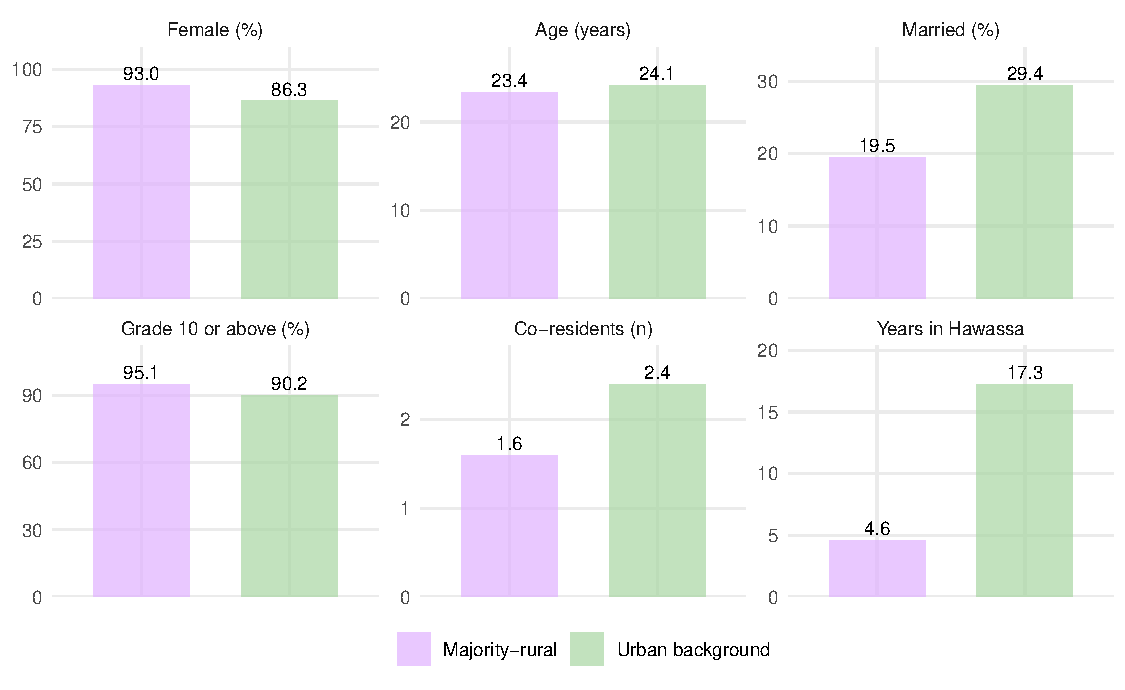
\includegraphics[width=0.8\textwidth]{../figures/fig_setting_demographics}
\fignote{A worker is majority-rural if more than half her life was spent in a rural area.}
\end{figure}

\noindent Workers were interviewed in person shortly after being hired. The median worker was interviewed \pnHireLagMedian{} days after her hire, with \pnHireWithinMonthPct{}\% reached within thirty days and \pnHireWithinTwoMonthPct{}\% within sixty. As mentioned previously, the intention of the design is to observe networks close to their point of formation. \\

\noindent Recruited workers come from a tight regional catchment, with \pnBornSidamaPct{}\% of our sample born in Sidama region, of which Hawassa is the capital (Appendix Figure~\ref{fig:catchment}).  We can infer that most of them are from the Sidama group, the majoritarian ethnicity in the region, a reading consistent with the fluency profile in Figure~\ref{fig:language}. The largest minority, \pnBornWolaytaPct{}\%, comes from Wolayta in the neighbouring South Ethiopia region. It is likely that this concentration has a political history. Hawassa formerly belonged to the multi-ethnic Southern Nations region, until a  referendum calling for Sidama's statehood passed in 2019. The following tensions discouraged workers of other ethnicities from coming to the park \citep{agarwal2026fieldnotes}. \\
\clearpage

\begin{figure}[h!]
\centering
\caption{Speaking fluency in Sidamigna and Amharic}
\label{fig:language}
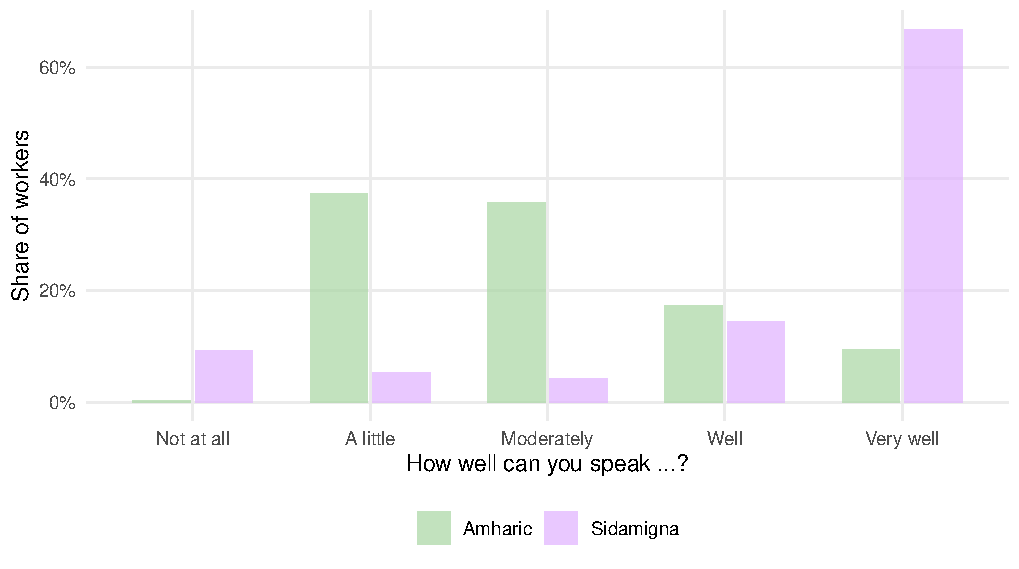
\includegraphics[width=0.8\textwidth]{../figures/fig_setting_language}
\end{figure}

\noindent Of sampled workers, \pnSidamaSpeakPct{}\% speak Sidamigna (the Sidama language, widely spokem in the country side) very well, while only \pnAmharicSpeakPct{}\% speak Amharic (nominally the Ethiopian lingua franca) at least well. Workers from Wolayta and elsewhere speak essentially no Sidamigna, so cross-group communication likely runs through weakly-held Amharic. \\

\noindent Workers all live in Hawassa, and are dispersed across Hawassa’s peri-urban kebeles\footnote{The smallest Ethiopian adminstrative unit, equivalent to a neighbourhood. Other administrative units are Region > Zone > Woreda > Kebele.} rather than concentrated near the park. Indeed, rents in Hawassa are too high relative to factory wages, and the park's own rental compounds are reported to take over half a monthly salary \citep{agarwal2026fieldnotes}. Workers commute by firm-provided bus or on foot. Co-workers feature predominantly as housemates, with \pnLiveCoworkerPct{}\% of workers living with at least one HIP co-worker. Urban-background workers more often live with relatives (Appendix Figure \ref{fig:housing}). \\

\noindent The median worker earns \pnWageMedian{} Birr a month at HIP\footnote{18 US dollars, August 2026 exchange rates}, with an interquartile range of \pnWagePTwentyFive{} to \pnWagePSeventyFive{} Birr (Appendix Table~\ref{tab:livelihoods}). Median household income over the previous three months (including the workers' own earnings, her partner's and any other member's) is \pnHhIncomeMedianThreeMo{} Birr.  The median reservation wage for an outside offer is \pnResvRatioMedian{} times her current wage. This tracks the market, as field informants put non-factory work in Hawassa (such as in services or construction) at around 5{,}000 Birr against 1{,}000-2{,}000 in the factories \citep{agarwal2026fieldnotes}. The worker spent a median of \pnDaysFindJobMedian{} days finding a job at HIP. \\

\noindent People working at HIP cannot live from their income: family transfers to workers are common precisely because the wage does not cover subsistence on its own \citep{agarwal2026fieldnotes}. On average, they are net receivers of financial help. Support comes from outside the factory. Other non-HIP contacts are the most common source,  while the home village follows. Transfers with co-hires exist but are the smallest on both margins. \\
\clearpage

\begin{figure}[h!]
\centering
\caption{Transfers by social group and direction, last 3 months.}
\label{fig:transfers}
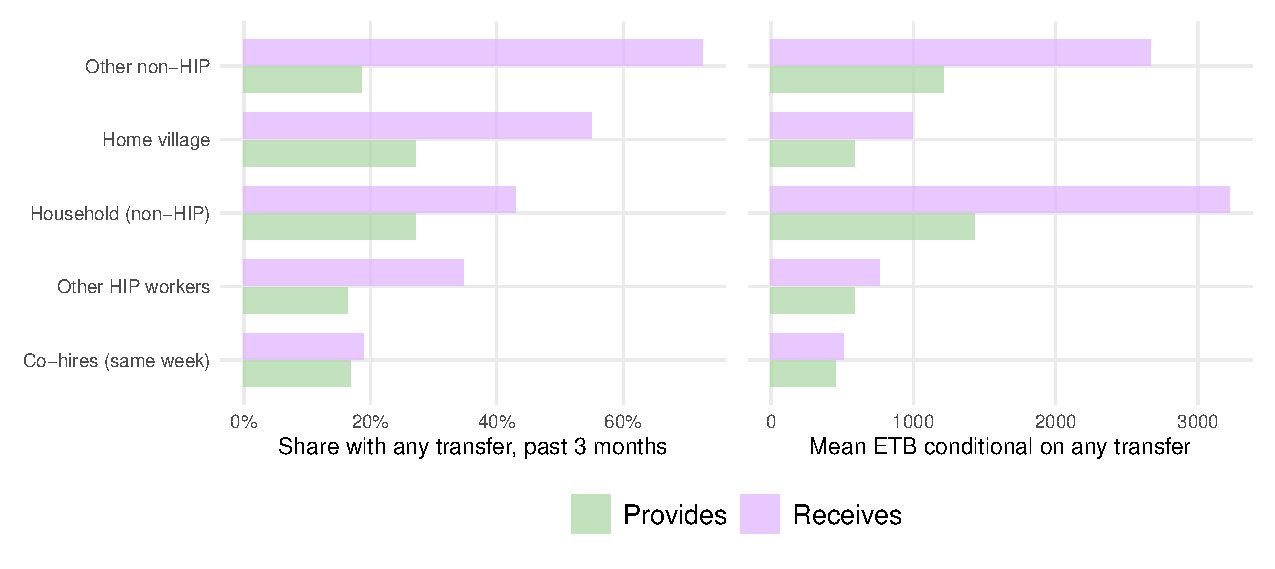
\includegraphics[width=\textwidth]{../figures/fig_setting_transfers}
\end{figure}

\noindent The median worker reports \pnMedNetworkWord{} network members, of which typically one is a co-hire (Figure~\ref{fig:network_size}). Co-hire ties tend to live in the workplace generators, such as breaks, friendship and commuting (Appendix Figure~\ref{fig:generators}). The money generators are answered mainly from the general network. \\

\begin{figure}[h!]
\centering
\caption{Network size per worker, by alter type}
\label{fig:network_size}
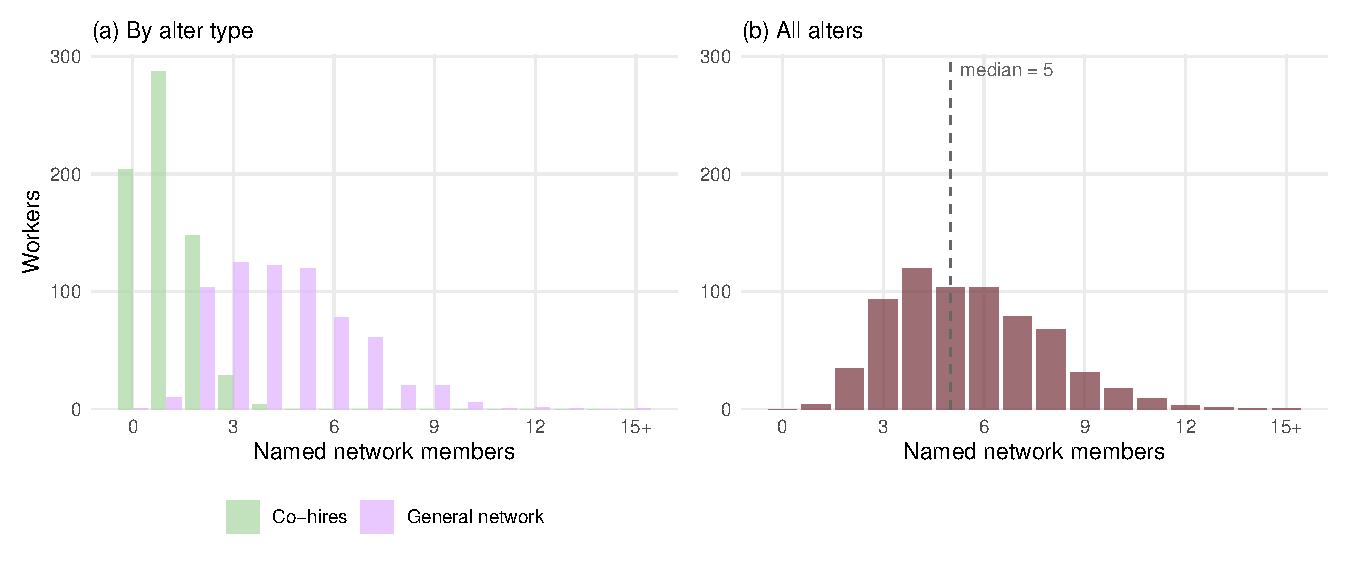
\includegraphics[width=\textwidth]{../figures/fig_setting_network_size}
\end{figure}

\clearpage
\parhead{On the recall of co-hires}

\noindent As mentioned previously, one of the first steps of the survey involves asking the respondent which ones of her co-hires she recalls. The median worker was trained with \pnRecallRosterMedian{} different people and recalled \pnRecallCountMedian{}, a median recall rate of \pnRecallRateMedianPct{}\%. \\

\noindent Of the \pnDyads{} pairs in which both members were themselves surveyed, \pnRecalledDyadPct{}\% are recalled and \pnTiedDyadPct{}\% are named on at least one of the fifteen layers. Given that a worker recalls a co-hire at all, she names her on some layer \pnTiedGivenRecalledPct{}\% of the time. The low tie rate is explained thus by the lack of recall. This suggests that people do not bond much over training. 

\begin{figure}[h!]
\centering
\caption{Recall rate against the number of names shown}
\label{fig:recall_roster}
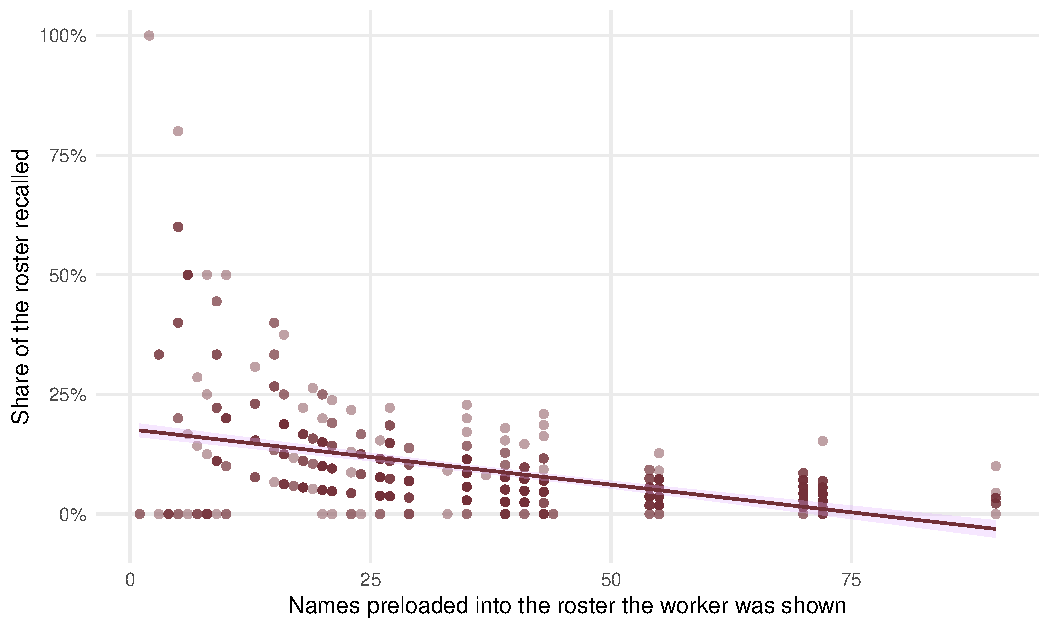
\includegraphics[width=0.8\textwidth]{../figures/fig_setting_recall_by_roster}
\fignote{One point is a worker; the line is the linear fit.}
\end{figure}

\noindent The recall rate falls in roster size, by \pnRecallSlopePerTen{} percentage points per ten additional names (Figure~\ref{fig:recall_roster}; $p = \pnRecallSlopeP{}$, heteroskedasticity-robust). This is driven by the denominator: across quartiles of roster size the median roster grows from \pnRecallRosterQOne{} names to \pnRecallRosterQFour{}, while the mean number recalled goes only from \pnRecallCountQOne{} to \pnRecallCountQFour{}. It appears as respondants have somehow a budget of about \pnRecallCountMedian{} people they can recall.\\

\parhead{On tie reciprocity of co-hires}

\noindent An important concern when working with this type of data is making sure we are recording real ties (and not noise). One way to check for this is what I call reciprocity - if A has nominated B, did B nominate A? On the \pnMutualPairs{} pairs where both workers were surveyed and each appeared on the other's roster, a report by one can be checked against the other. \\

\noindent I expect some relationship layers to be mutual, and other to be more directional. Layers more mutual by nature (\textit{e.g.} commuting together, taking breaks together) reciprocate at \pnRecipReciprocalPct{}\% pooled. Layers such as asking for advice or receiving money reciprocate at \pnRecipDirectionalPct{}\% (Table~\ref{tab:reciprocity}, Figure~\ref{fig:reciprocity}). Co-hire recall itself reciprocates at \pnRecipRecallPct{}\%. 

\begin{table}[h!]
\centering
\caption{Reciprocity by layer}
\label{tab:reciprocity}
\small% GENERATED by "14 descriptives - recall.R" - do not edit by hand.
\begin{tabular}{lrrr}
\textit{layer} & \textit{reported} & \textit{confirmed} & \textit{reciprocity} \\
\dmidrule
\multicolumn{4}{l}{\textit{Expected reciprocal}} \\
\quad Co-hire recall & 1{,}203 & 432 & 36\% \\
\quad Navigate hawassa & 205 & 48 & 23\% \\
\quad Commute & 287 & 98 & 34\% \\
\quad Meet outside work & 209 & 58 & 28\% \\
\quad Call or text & 275 & 82 & 30\% \\
\quad Workplace breaks & 413 & 124 & 30\% \\
\quad Friends & 355 & 110 & 31\% \\
\quad Rosca ekub & 21 & 0 & 0\% \\
\addlinespace
\multicolumn{4}{l}{\textit{Expected directional}} \\
\quad Advice personal decision & 209 & 38 & 18\% \\
\quad Borrow money (in) & 217 & 30 & 14\% \\
\quad Large expenses (in) & 43 & 0 & 0\% \\
\quad Job search & 174 & 26 & 15\% \\
\quad Assistance (in) & 103 & 18 & 18\% \\
\quad Borrow money (out) & 79 & 4 & 5\% \\
\quad Large expenses (out) & 7 & 0 & 0\% \\
\quad Assistance (out) & 22 & 0 & 0\% \\
\bottomrule
\end{tabular}

\fignote{Restricted to the \pnMutualPairs{} pairs in which each worker appeared on the other's roster. \textit{Reciprocity} is \textit{confirmed} over \textit{reported}.}
\end{table}

\begin{figure}[h!]
\centering
\caption{Reciprocity by layer and expected direction}
\label{fig:reciprocity}
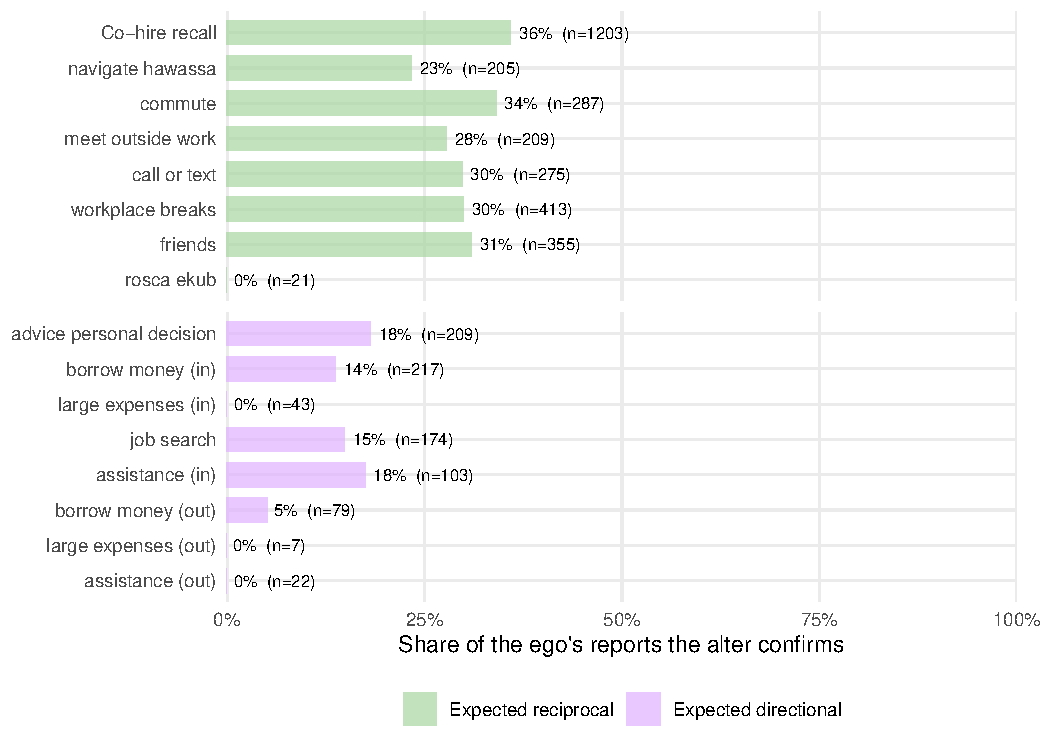
\includegraphics[width=0.85\textwidth]{../figures/fig_setting_reciprocity}
\end{figure}
\clearpage

\noindent Note that risk-sharing layers have low mentions and low reciprocity rates because, as seen in Figure~\ref{fig:transfers}, these are more general network relationships. This sections only looks at co-hires, as it is the only category we can verify. \\

\parhead{On the inheritance of ties}

\noindent Even if this section is descriptive, it starts to document the answer to my questions. Indeed, we can see that network workers report is overwhelmingly inherited. On average, \pnPreHipSharePct{}\% of named alters were known before joining HIP, and \pnPreHipHalfPct{}\% of workers knew at least half of their named network from before entry. The distribution is  more concentrated for urban-background workers than for the majority-rural (Figure~\ref{fig:inherited}). \\

\begin{figure}[h!]
\centering
\caption{Cumulative distribution of pre-HIP share, by background.}
\label{fig:inherited}
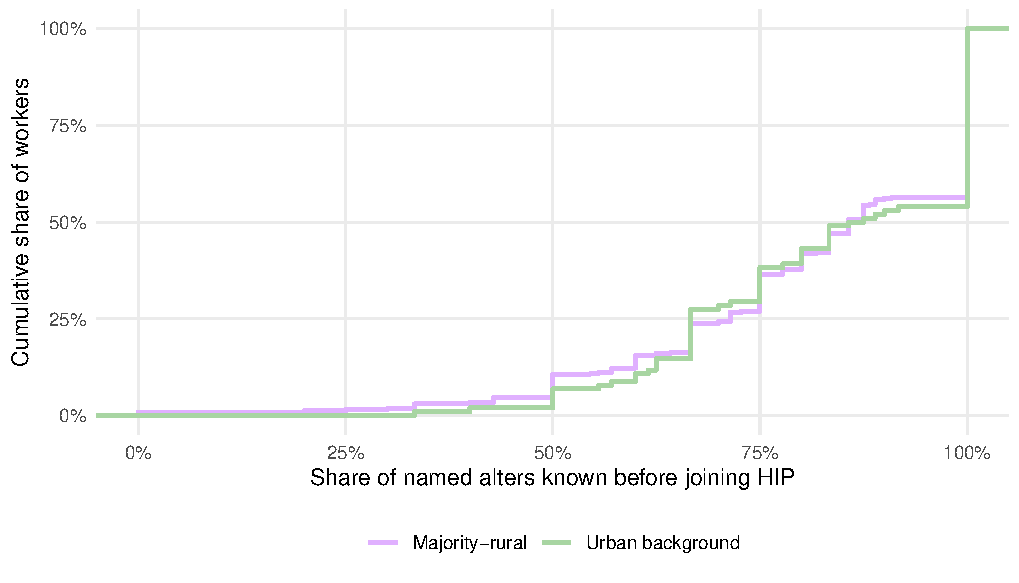
\includegraphics[width=0.8\textwidth]{../figures/fig_setting_inherited}
\end{figure}

\noindent This is not only driven by the general network, as we may expect\footnote{As a reminder, co-hire ties are between two workers, whereas general-network alters are described only by the respondent and are mostly not HIP employees.}.  About \pnTieCohireInheritedPct{}\% co-hire ties are inherited (\pnTieCohireInherited{} of them), against \pnTieGnInheritedPct{}\% of general-network ties (\pnTieGnInherited{}). Inherited co-hire ties are \pnTieCohireFriendPct{}\% friendships, against \pnTieCohireKinPct{}\% kin. In the general network the split is \pnTieGnKinPct{}\% kin against \pnTieGnFriendPct{}\% friends. It appears as the inherited general network is the origin community, while the inherited part of the co-hire network is a thinner and more geographically dispersed set of friendships (Table~\ref{tab:tie_composition}). \\

\begin{table}[h!]
\centering
\caption{Composition of inherited ties, by roster}
\label{tab:tie_composition}
% GENERATED by "16 descriptives - ties and dyads.R" - do not edit by hand.
\begin{tabular}{lrrr}
& \textit{ties} & \textit{\% of inherited} & \textit{\% co-villager} \\
\dmidrule
\multicolumn{4}{l}{\textit{Co-hire ties}} \\
Kin & 37 & 12.2 & 55.6 \\
Friends & 231 & 76.2 & 20.6 \\
Acquaintances & 35 & 11.6 & 9.1 \\
\midrule
\multicolumn{4}{l}{\textit{General network}} \\
Kin & 1{,}450 & 52.2 & 86.9 \\
Friends & 1{,}206 & 43.4 & 48.3 \\
Acquaintances & 122 & 4.4 & 25.6 \\
\bottomrule
\end{tabular}

\fignote{One observation is an inherited tie; shares are within roster. \textit{Kin} covers all family codes (1--6). \textit{\% co-villager} is the share born in the worker's own woreda, over ties with a usable origin code.}
\end{table}

\noindent On a side note, it appears as information about the job travels to the general network. Even if \pnJobInfoNonePct{}\% of the analysis sample (\pnJobInfoNone{} of \pnAnalysisN{} workers) report that they gathered information about jobs in the Park from no one, the remaining \pnJobInfoEgos{} name \pnJobInfoTies{} general-network informants. These informants are \pnJobInfoFriendPct{}\% friends and \pnJobInfoKinPct{}\% kin. \\

\FloatBarrier
\parhead{On the depth and multiplexing of ties}

\noindent As suggested before, a relationship is rarely one thing at a time. The friend you commute with may also be the one you confide in, and your landlord might very well be your partner. This is dubbed a multiplex network. In our sample, \pnMuxCohireTwoPct{}\% of co-hire ties span at least two layers and \pnMuxCohireSixPct{}\% span six or more. For general-network ties,  \pnMuxGnTwoPct{}\% are multiplex and \pnMuxGnSixPct{}\% span six or more layers (Figure \ref{fig:multiplex}). \\

\begin{figure}[h!]
\centering
\caption{Number of ties each alter appears in, by type}
\label{fig:multiplex}
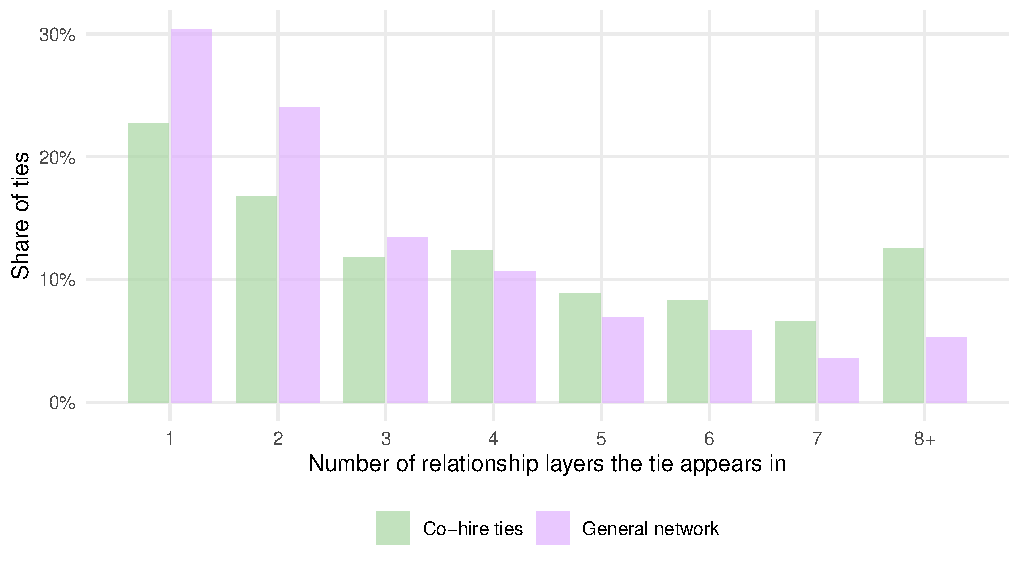
\includegraphics[width=0.8\textwidth]{../figures/fig_setting_multiplex}\end{figure}
\FloatBarrier

\noindent The question becomes which ties are grouped together, or which type of relationships are usually multiplex. Figure~\ref{fig:cooc} analyses the fifteen layers pairwise. A cell is the probability that a tie already carrying the row layer also carries the column layer. \\

\begin{figure}[h!]
\centering
\caption{Which relationship layers travel together? Conditional Probability}
\label{fig:cooc}
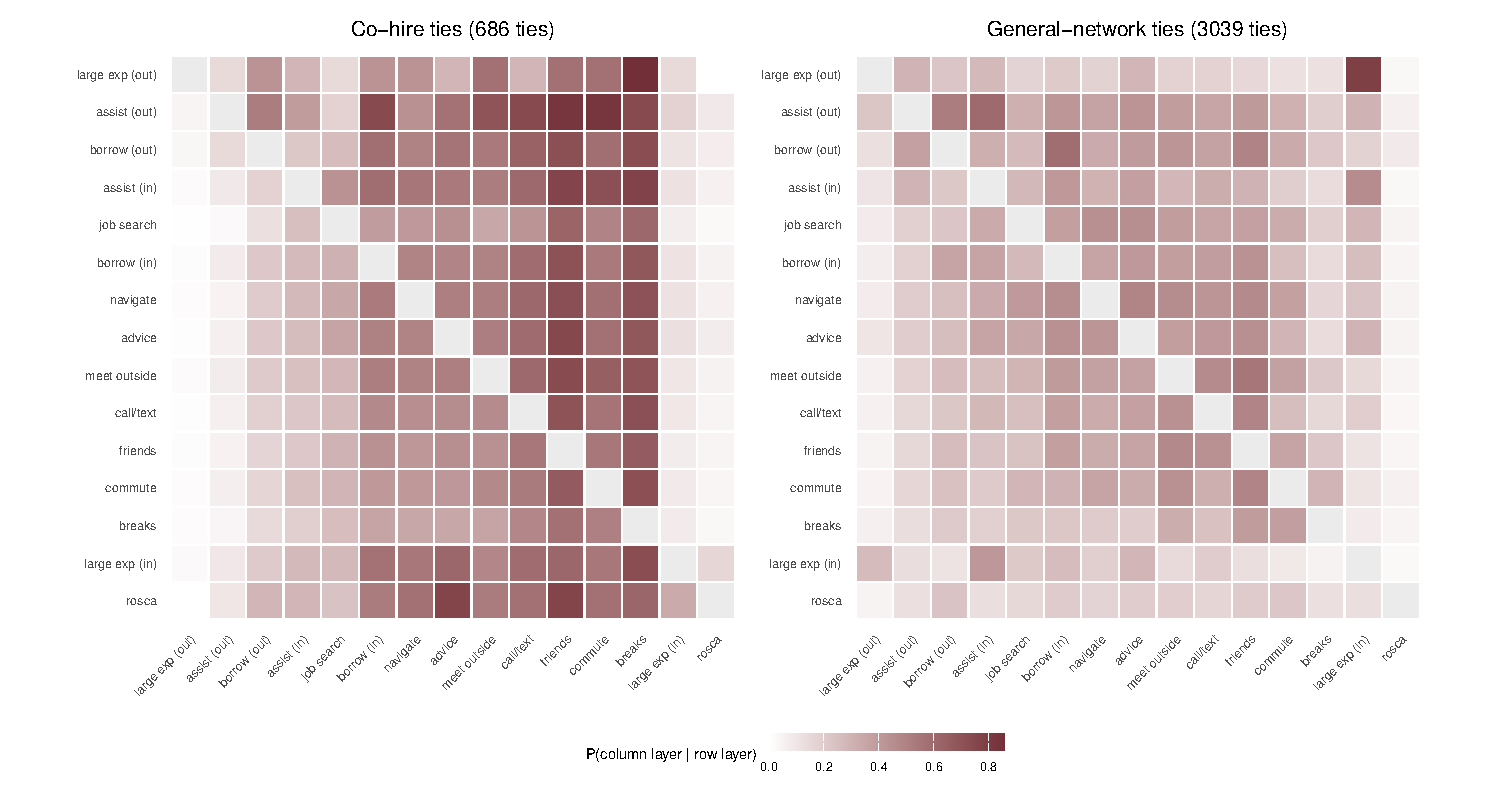
\includegraphics[width=\textwidth]{../figures/fig_setting_layer_cooc_cond}
\fignote{A cell is the share of ties carrying the row layer that also carry the column layer, so the matrix is asymmetric. \textit{large expenses (out)}, \textit{Rosca} and \textit{large expenses (in)} rest on \pnThinLargeExpOut{}, \pnThinRosca{} and \pnThinLargeExpIn{} ties; their rows read dark only because those \pnThinLargeExpOutWord{} ties are dense ones.}
\end{figure}
\FloatBarrier
\noindent Co-hire relationships are thinner than the general network, which makes sense since they are no older than the worker's tenure at HIP. Among co-hire ties, a tie carrying one layer associated to companionship (commuting, breaks, friendship, meeting outside work, calling) carries another given companionship layer with probability \pnCondCompCohire{} (\pnCondCompGn{} for the general network), but carries any given risk-sharing outflow with probability \pnCondOutCohire{} (\pnCondOutGn{} for the general network). Only \pnAnyOutCohirePct{}\% of co-hire ties carry some risk-sharing outflow overall (\pnAnyOutGnPct{} for the general network), and \pnAnyOutCommuteCohirePct{}\% of those that carry commuting do (\pnAnyOutCommuteGnPct{} for the general network). \\

\parhead{Observations}

\noindent We have now a clear picture of the environment these people evolve in. People remain tied to their origin community and inherit \pnTieCohireInheritedPct{}\% of the colleagues they name at work. They do not recall many people from their trainings, and form new ties for company rather than for risk-sharing. A month after arriving, her usable network is essentially the one she brought with her. \\

\noindent The set-up that follows in the next section is minimal. Its purpose is to show that the aforementioned four channels can be thought as parameters of a same model. It allows me to identify what I can try to estimate. 



\newpage
\section{Toy model}
\label{sec:model}
\noindent Let there be a multitude of workers. Each worker $i$ has origin $o_i$, identified at the woreda level (an Ethiopian administrative unit, corresponding to a village and its surroundings) and carries a language endowment. She has been hired at HIP in a \textit{hiring batch} $b_i$ and, after training, assigned to a \textit{production unit} $p_i$. 
\[
h_{ij} = \mathds{1}\{o_i = o_j\}, \qquad
s_{ij} = \mathds{1}\{i,j \text{ share a language}\}, \qquad
u_{ij} = \mathds{1}\{p_i = p_j\}
\]
for a shared origin, a shared language, and a shared production unit. These characteristics will help me understanding if people are drawn to others who share their same references, if they seek someone with which they can communicate well, or if they befriend whoever they are exposed to repeatedly. \\

\noindent There are two periods. Period 0 represents life before the Park, while period 1 is the Park at the moment of the survey. I write $g^0_{ij}$ for a tie that is formed at period 0, \textit{i.e.} that already exists before either worker is recruited, and $g^1_{ij}$ for one formed inside the Park. Ties persist through time, thus a tie made in Period 0 will be carried over in Period 1. \\

\parhead{Ties formed in Period 0}

\noindent Let us focus on $g^0_{ij}$. Same-origin pairs are likelier to arrive already acquainted, and conversely pairs who are already acquainted are likelier to arrive together. To model this, I set that in Period 0,  the pair is linked with probability
\begin{equation}
\label{eq:model-inherit}
\Pr(g^0_{ij}=1) \;=\; \pi_0 + \pi_1 h_{ij}, \qquad \pi_1 > 0,
\end{equation}
where $\pi_0$ is the baseline chance that two workers know each other, and $\pi_1$ is the chance that two workers are acquainted when we consider two people of the same woreda. The $\pi_1$ is somehow a "chance premium", and is positive.\\

\noindent To account for the fact that workers are likely not sorted independently, I introduce the parameter $\rho \geq 1$. It is the factor by which knowing each other in Period 0 raises the odds that two concerned workers share a batch. Note that $\rho = 1$ is when batches are blind to the existing network, $\rho > 1$ is when batches travelling along it. The \textit{importation channel} is thus captured by the pair $(\pi_1, \rho)$, with the first capturing the fact that inherited ties will be homophilous, and the second deciding how many of those ties translate into co-hires. \\

\parhead{Ties formed in Period 1}

\noindent Let us now turn to pairs with $g^0_{ij}=0$, who arrive at HIP as strangers. For a tie to form , two things must happen in order:
\begin{enumerate}
    \item the two workers must meet,
    \item $i$ must name $j$, or the contrary, or both. \footnote{The second step can one-sided. As we will see, there are unreciprocated ties, and the exclusion channel below is read entirely from the difference between $i \to j$ and $j \to i$.}.
\end{enumerate}
\noindent I take these in turn. The survey used sees only the two steps together, since it asks a worker whom she names and never whom she met. A name
not produced may have failed at either step. \\

\noindent The first step involves meeting the other person. Two co-hires interact with probability
\begin{equation}
\label{eq:model-meet}
m_{ij} \;=\; \big[\, \mu_b \;+\; \mu_p\, u_{ij} \,\big]\, \kappa^{\,1-s_{ij}},
\qquad \mu_b > 0,\;\; \mu_p > 0,\;\; \kappa \in [0,1],
\end{equation}
This is the \textit{opportunity channel}, and it has three parts. First,
$\mu_b$ is the chance that any two batch-mates meet at all, whatever else
they have in common. Second, $\mu_p u_{ij}$ adds to that chance when the
two share a production unit. Third, the factor $\kappa^{\,1-s_{ij}}$ discounts pairs with no language in common. It equals one when they share a language and $\kappa$ when they do not. The idea is that undergoing training together adds occasions to meet, while having no language in common scales down every occasion that the pair has. Note that origin is not included in the opportunity channel\footnote{This implies that once
production unit and language are accounted for, meeting inside the Park is
blind to origin.}, to distinguish it from the taste channel.  \\

\noindent The second step involves having an actual tie with the other person.  If two workers have met, $i$ will name $j$ when
\begin{equation}
\label{eq:model-name}
n_{ij} \;=\; \mathds{1}\big\{\, \alpha_i + \gamma_{ij} + \tau\, h_{ij} + \varepsilon_{ij} > 0 \,\big\},
\qquad
\gamma_{ij} \;=\; \bar{\gamma}_j - \delta\, \mathds{1}\{j \in \text{minority}\}\,\mathds{1}\{i \notin \text{minority}\},
\end{equation}

\noindent where $\varepsilon_{ij}$ is noise. Following \citet{graham2017econometric}, $\alpha_i$ is how freely $i$ names anyone at all and $\bar{\gamma}_j$ how readily $j$ is named by anyone. The \textit{taste channel} is $\tau$, the premium a worker attaches to a partner from her own woreda. The \textit{exclusion channel} is $\delta \geq 0$, \textit{i.e.} the lower chance that a majority worker nominates a minority one. Note that, in this context, I define minority as an individual who was either born outside of Sidama region\footnote{This represents \pnChanMinorityRegionN{} of the \pnAnalysisN{} workers.} or who reports speaking little to no Sidamigna\footnote{This is \pnChanMinorityLangN{} workers.}.  The two agree on \pnChanMinorityBothN{} workers. \\

\noindent It is not immediate how to separate taste from exclusion. What I propose is to argue that taste is a characteristic of the pair, while exclusion is directional. Since $h_{ij} = h_{ji}$, the taste term $\tau h_{ij}$ enters the nomination $i \to j$ and the nomination $j \to i$ identically. On the other hand, exclusion does not. If $j$ is a minority worker and $i$ is not, then $i \to j$ carries the penalty $-\delta$ while $j \to i$ carries nothing.\\

\noindent Putting the two steps together, a worker who arrived a stranger
names $j$ with probability
\[
\Pr(g^1_{ij}=1) \;=\; m_{ij} \cdot
\Pr\big(\alpha_i + \gamma_j + \tau\, h_{ij} + \varepsilon_{ij} > 0\big).
\]
Thus who workers recall or not, who they nominate or not, is a result of those forces.  \\

\noindent Table~\ref{tab:mapping} collects the four channels, the
parameters that carry each of them, what each would leave behind in the
network if it were the one at work, and the specification of
Section~\ref{sec:strategy} that goes looking for it. \\

\begin{table}[h!]
\centering
\caption{The four channels, and where each is tested}
\label{tab:mapping}
\footnotesize
\begin{tabular}{lllp{0.34\textwidth}l}
\textit{channel} & \textit{parameter} & \textit{where it acts} & \textit{signature in the network} & \textit{test} \\
\dmidrule
importation & $\pi_1, \rho$ & before HIP & the same-origin premium loads on ties that predate the batch, not on those formed in it & Spec.~2 \\
\medskip
opportunity & $\mu_p, \kappa$ & meeting & ties follow the production unit or the shared language & Spec.~3 \\
\medskip
taste & $\tau$ & naming & a same-origin premium on ties formed at HIP, and a tilt in what those ties are used for & Spec.~4, 8 \\
\medskip
exclusion & $\delta$ & naming & minority workers named less \textit{by the majority}, and their nominations returned less often & Spec.~5 \\
\bottomrule
\end{tabular}
\end{table}
\FloatBarrier

\parhead{Comment}

\noindent In the next section, I try to make the parameters of the model empirically testable. My toy model is not performant in predicting the outcomes we will discuss in Section \ref{sec:results}. Attempting to model a priori the homophily creation process, however, provided me with insights that were then indeed validated. In particular, splitting ties by period, or looking at ties in a directional manner, made for informative regressions.

\newpage
\section{Empirical Strategy}
\label{sec:strategy}

\parhead{On the limitations of a more robust design}

\noindent The empirical specifications I have implemented in this thesis are unfortunately not causal. I chose not to attempt a causal design, as I believed the needed assumptions did not hold. \\

\noindent Ideally, I could have exploited the fact that workers do not choose their batch - they are hired with whoever else was hired that week. It could be argued that, given the setting, a worker's exposure to particular kinds of colleague is exogenous and can be regressed directly on her outcomes. For example, the origin composition of her batch could be a predictor of how homophilous her network becomes. Similarly, the share of a worker's co-hires who come from an urban background could be a predictor of who she ties with (and what her outcomes) are. \\

\noindent After performing a series of tests, reported in Appendix~\ref{sec:appendix-quasirandom}, I have chosen not to go down this route. I find that belonging to a certain batch predicts several individual charateristics, probably because individuals migrate and get hired together. One of the tests finds that a worker's co-hires are drawn from her own woreda \pnWoredaExcessPct{}\% more often than her firm's composition implies, and this excess survives holding the firm fixed\footnote{Because one of the reasons could have been that firms hire from different catchments.}. My understanding is that to perform the above-mentioned design, I would have needed for batch composition to be exogenous variation, \textit{i.e.} for the composition of a batch to carry no information about the worker hired into it. \\

\noindent Additionally, my data is cross-sectional, which rules out exploiting a time dimension or following people as they tie with colleagues assigned to their production unit. Given that they are allocated to units according to how they performed during the training, that specific assignement could be considered exogenous if performance is assumed independent from origin. \\

\noindent In the models below, every specification is therefore estimated within batch, so that the comparison is between workers, or pairs of workers, who were handed the same set of colleagues. What differences remain across batches are absorbed. \\

\parhead{Extensive margin}

\noindent The first specifications I test are linear probability models (LPM). They assess what is correlated with the existence of a tie. These are flexible and straightforward to interpret. The models below recover the probability of a tie (or rather, the linear projection rather than the probability itself). As happens with linear projections, the estimates can leave the [0,1] interval. Note that in my exercise, at worst \pnChanLpmOutsidePct{}\% of pairs in a specification do, almost all of them below zero, and never by more than \pnChanLpmMaxDevPp{} points. \\

\noindent A logit fits the same data with a curve rather than a line, and the curve is bounded, so none of its fitted values can fall outside the interval. Its coefficients are log-odds and not probabilities (which is less convenient), and it drops all observations in batches in which nobody forms a tie, which does not happen with the LPM\footnote{The logit drops the whole batch, because due to the fixed effects each batch essentially enters as its own dummy. In a batch where nobody tied, the dummy enters as 0 and the likelihood has no finite maximum. A logit then estimates the effect among the batches where ties happened rather than among all of them, but it thus obscures a part of the story - why did those people not tie ?}. \\

\noindent In any case, I have estimated most equations with a logit to see if results would differ substantially, and they do not (Table~\ref{tab:logit}).  Across the extensive-margin equations, no coefficients change sign or significance. The logit discards \pnChanLogitDropBatches{} of the \pnChanLogitBatches{} batches. As a consequence, I decided to use the LPM specification throughout. \\

\noindent \underline{\textit{Specification 1: Recall}} \\[0.4em]
I first investigate what is associated with recall. This regression gives clues on which of the four channels is the most promising. \\ 

\noindent Writing $\text{recalled}_{ij}=1$ when $i$ produced $j$'s name,
\begin{equation}
\label{eq:strategy-recall}
\begin{split}
\text{recalled}_{ij} \;=\; \theta_1\,\text{same woreda}_{ij} \;&+\; \theta_2\,\text{same unit}_{ij} \\
&+\; \theta_3\,\text{shared language}_{ij} \;+\; \lambda_{b} \;+\; \varepsilon_{ij},
\end{split}
\end{equation}
where $\theta_1$ to $\theta_3$ are what each feature adds to the chance of being recalled and $\lambda_b$ is a batch fixed effect. The batch FE holds fixed the roster the worker was handed, but absorbs the intercept. The variation used is thus within batch, \textit{i.e.} pairs drawn from the same roster that differ in whether the two members share a woreda, share a production unit\footnote{\noindent The production unit is unrecorded for one member of the pair or both in \pnPuUnknownPct{}\% of pairs. Rather than drop them, I set the indicator to
zero for them and enter a second indicator for the unit being unrecorded beside it. That second indicator carries its own intercept, so the zeros I inserted sit in a group of their own and $\theta_2$ is read off the pairs whose units are observed. Dropping them instead would estimate this equation on a smaller sample than the ones that do not involve the production unit, and the coefficients on \textit{same woreda} and \textit{shared language} would no longer be comparable across specifications. }, or can speak to one another. \\

\noindent This is valid, but potentially biased towards zero. I began to be concerned with the idea that people have a "budget" in recall. If the training is a place where we make rather shallow connections, then I will recall a limited number of people. If there is such budget, a feature that raises the chance one co-hire is named lowers it for the others. I abstract from this for now. \\

\noindent \underline{\textit{Specification 2: Importation}} \\[0.4em]
If a network is imported, the same-origin premium sits on ties that predate the batch.\\

\noindent The test is a regression of \textit{inherited tie} on the same-origin indicator
\begin{equation}
\label{eq:strategy-import}
\text{inherited tie}_{ij} \;=\; \pi_1\,\text{same woreda}_{ij} \;+\; \pi_2\,\text{same zone}_{ij} \;+\; \lambda_{b} \;+\; \varepsilon_{ij},
\end{equation}
where $\pi_2$ is what sharing the coarser geography adds to the chance that two workers arrived already acquainted and $\lambda_b$ is a batch fixed effect. Because the zone is held fixed alongside it, $\pi_1$ is the premium for a shared woreda specifically, in addition to what a shared zone already buys. The variation used is again within batch\footnote{And for $\pi_1$, it is narrower still. It is pairs who share a zone but differ in whether they also share a woreda.}.  \\
\clearpage


\noindent \underline{\textit{Specification 3: Opportunity}} \\[0.4em]
To isolate opportunity, I must exploit something that shifts the meeting technology without being preferences. The candidates are the production unit the firm assigns after training, and whether two workers share a language\footnote{Neither is ideal. Units are assigned after training and on the basis of performance, so two workers placed together may be alike in ways I do not observe. Language could technically fall into taste for one's own group, but you may have people from a different group fluent in one or more languages that you speak.}. \\

\noindent Restricting attention to the pairs who arrived as strangers, so that the outcome is whether they went on to be tied inside the Park,
\begin{equation}
\label{eq:strategy-opp}
\text{new tie}_{ij} \;=\; \mu_p\,\text{same unit}_{ij} \;+\; \beta_s\,\text{shared language}_{ij} \;+\; \lambda_{b} \;+\; \varepsilon_{ij},
\end{equation}
 where $\mu_p$ is what the firm's placing the two together in a production unit adds to the chance of a tie and $\beta_s$ is what a language in common adds to it. The variation used is within batch and among the pairs who arrived as strangers. \\


\noindent \underline{\textit{Specification 4: Taste}} \\[0.4em]
On pairs who arrived as strangers, I can see whether there is a same-origin premium in the ties they went on to form. 
\begin{equation}
\label{eq:strategy-taste-cohire}
\begin{split}
\text{new tie}_{ij} \;=\; \tau\,\text{same woreda}_{ij} \;&+\; \mu_p\,\text{same unit}_{ij} \;+\; \beta_s\,\text{shared language}_{ij} \\
&+\; \alpha_i \;+\; \gamma_j \;+\; \varepsilon_{ij}.
\end{split}
\end{equation}
\noindent Unit assignement and language enter again as controls. There is no intercept, because the sender effect $\alpha_i$ (how freely the respondent names anyone) and the receiver effect $\gamma_j$ (how readily the alter is named by anyone) absorb it. What is left on \textit{same woreda} is a premium attached to the pair. The variation used is within respondent and within alter. The coefficient $\tau$ is read off the co-hires a single worker was presented with, who differ in whether they come from her woreda. I estimate the same equation a second time with \textit{same zone} in place of \textit{same woreda}. It is better powered, since many more pairs share a zone than share a woreda.  \\

\noindent \underline{\textit{Specification 5: Exclusion}} \\[0.4em]
Refusal is a property of the person refused, is directional, and might carry information. It is captured empirically by the receiver effect ${\gamma}_j$ of equation ()\ref{eq:strategy-taste-cohire}), and I try to assess here if it can be predicted by minority status. \\

\noindent I estimate $\delta$ on the dyads, letting the namer's own status enter,
\begin{equation}
\label{eq:strategy-excl-split}
\text{new tie}_{ij} \;=\; -\,\delta\,\text{minority}_j \;-\; \psi\,\text{minority}_j \times \text{minority}_i \;+\; x_{ij}'\beta \;+\; \lambda_b \;+\; \varepsilon_{ij},
\end{equation}
where $x_{ij}$ carries the same shared-woreda, same-unit and shared-language controls as Specification 3. Here $\delta$ is read only off pairs whose namer is \textit{not} a minority worker, which is the quantity the model defines, and $\psi$ says how that penalty changes when the namer is a minority worker too. Both enter negatively, so a positive $\delta$ is a penalty. \\

\noindent This might have power problems, since $\delta$ is identified only off the \pnChanExclOutPairs{} pairs in which exactly one member is a minority worker. \\

\noindent Standard errors in equations~\eqref{eq:strategy-recall} to~\eqref{eq:strategy-taste-cohire} are clustered on both members of the pair, since a worker appears in as many rows as she has co-hires and on both sides of them. Equation~\eqref{eq:strategy-excl-split} is estimated on the dyads directly and is clustered the same way. \\

\parhead{Intensive margin}

\noindent The specifications above ask whether a tie exists. The ones below condition on a tie existing and ask what determines the quality and the quantity of its layers. Specification 6 asks whether a tie to someone from home does more. Specification 7 asks whether the ties a worker brought with her are used for different things than the ones she made here. Specification 8 asks whether a shared origin redistributes a tie across functions without changing how many it carries.\\

\noindent Note that in Specifications 6 and 7 an observation is a tie and the fixed effect is the worker, so that every comparison is between two ties of the same person. In Specification 8 an observation is a tie on one of the fifteen layers and the fixed effect is the pair. \\


\noindent \underline{\textit{Specification 6: Depth}} \\[0.4em]
Let me write $\text{layers}_{ij} = \sum_q \text{tie}_{ijq}$ for the number of the fifteen layers a tie carries, and $\text{knew before}_{ij}=1$ when the tie is inherited. I ask what determines how much a tie carries, counting the fifteen layers as interchangeable:
\begin{equation}
\label{eq:strategy-depth}
\begin{split}
\log \mathbb{E}\big[\text{layers}_{ij}\big] \;=\; \omega_1\,\text{knew before}_{ij} \;&+\; \omega_2\,\text{same woreda}_{ij} \;+\; \omega_3\,\text{shared language}_{ij} \\
&+\; \omega_4\,\text{same unit}_{ij} \;+\; \alpha_i,
\end{split}
\end{equation}
estimated by Poisson, so each $\omega$ reads as a proportional change in the number of layers rather than as a count. Thus, $\omega_1$ is what a tie's predating the Park does to its depth, $\omega_2$ what a shared woreda does, $\omega_3$ what a language in common does and $\omega_4$ what the firm's having placed the two together does. $\alpha_i$ is a respondent effect.\\

\noindent Note that the count has no zeros by construction, because a tie is in the sample only if it carries at least one layer. Also, with $\alpha_i$, the variation used is between two ties of the same worker that differ in vintage, in origin, in language or in production unit - thus workers with a single recorded tie are collinear and drop out. Standard errors are clustered on both members of the pair on the co-hire roster, and on the respondent alone for the few analyses on the general network.\\

\noindent The sample is ties, so whatever selects a pair into having a tie selects it into this regression. This generates bias, the direction of which is unclear. A selection model on tie existence could in theory address it (and I have attempted it), but I believe the exclusion restriction did not hold. I try to get a sense of selection by adding indicators and interactions for \textit{kin} and \textit{friend}, and with $\alpha_i$ replaced by a constant so as to observe the respondent effect. \\

\noindent \underline{\textit{Specification 7: Vintage}} \\[0.4em]
I ask whether imported ties differ in tie content. For each layer $q$ separately,
\begin{equation}
\label{eq:strategy-vintage}
\text{tie}_{ijq} \;=\; \sigma_q \, \text{knew before}_{ij} \;+\; \alpha^{q}_{i} \;+\; \varepsilon_{ijq},
\end{equation}
a linear probability model with a respondent effect, estimated one layer at a time. Thus, $\sigma_q$ is how much likelier an old tie is than a new one to be used for that particular dimension. \\

\noindent There are fifteen tie layers, translating in fifteen sets of respondent effects. The variation used for $\sigma_q$ is ties of the same worker that differ in vintage. Standard errors are clustered on the worker. \\

\noindent \underline{\textit{Specification 8: Multiplexing}} \\[0.4em]
I ask whether shared origin tilts  the tie toward some functions and away from others. Stacking the tie-by-layer observations,
\begin{equation}
\label{eq:strategy-layer}
\text{tie}_{ijq} \;=\; \sum_{q} \beta_q \big( \text{same woreda}_{ij} \times \mathds{1}\{q\} \big) \;+\; \psi_{q} \;+\; \zeta_{ij} \;+\; \varepsilon_{ijq},
\end{equation}
where $\beta_q$ is how much a shared woreda shifts the tie toward layer $q$, with one coefficient per layer. Layer fixed effect $\psi_q$ absorbs how common that layer is across all ties, and $\zeta_{ij}$ is a fixed effect for the pair. \\

\noindent The design absorbs everything that is a property of two people rather than of a function. Note that a consequence is that the fifteen coefficients are pinned only relative to one another and are reported as deviations from their own mean. This design cannot say whether a shared origin makes a tie carry more layers, only how it spreads them across the fifteen. A flat profile says that taste does not shape what a tie is used for, independently of what it does to whether the tie exists at all. \\

\noindent Kinship can load onto $\beta_q$. I estimate equation~\eqref{eq:strategy-layer} a second time with kinship given fifteen interactions of its own, $\beta^{\text{kin}}_q$, so that the two profiles are fitted side by side. If the two trace the same shape across the fifteen layers, then origin is simply kinship.\\

\clearpage
\section{Results}
\label{sec:results}

\parhead{Extensive margin}

\noindent \underline{\textit{Specification 1: Recall}} \\[0.4em]
It appears that shared origin raises recall mostly because those specific ties were imported. Sharing a woreda increases the recall probability by \pnChanRecallOriginPp{} percentage points on a base recall rate of \pnChanRecallBasePct{}\%, and this falls by more than half when excluding imported ties. Indeed, same-woreda pairs are far likelier to be among those \pnChanRecallPreTied{} inherited pairs. \pnChanRecallPreWoredaPct{}\% of them arrived acquainted, against \pnChanRecallPreOtherPct{}\% of the rest (Table \ref{tab:recall}). \\[-0.6em]

\noindent Among strangers, sharing a production unit increases the recall probability by \pnChanRecallUnitStrPp{} points. This is likely driven by people who have completed the training, and receive daily exposure to the alter. A language in common indeed raises recall, by \pnChanRecallLangStrGain{} percentage points, likely through more interaction opportunities. \\

\noindent \underline{\textit{Specification 2: Importation}} \\[0.4em]
As seen above, shared origin predicts an inherited tie strongly. A shared woreda raises the chance that two workers arrived already acquainted by \pnChanImportOriginPp{} percentage points on a base rate of \pnChanImportBasePct{}\%\footnote{That premium is \pnChanImportMult{} times the base rate itself, so it multiplies the chance by \pnChanImportOriginRel{}.} (Table~\ref{tab:tie_formation} ). People seem to import hyperlocal ties, as sharing a zone is not as predictive of a tie. \\

\noindent \underline{\textit{Specification 3: Opportunity}} \\[0.4em]
Among the \pnChanNewN{} pairs who arrived as strangers, it appears as some ties are indeed shaped by the opportunity channel. If the firm has placed two workers in the same production unit, this raises the chance they form a tie by \pnChanOppUnitPp{} percentage points on a base of \pnChanOppBasePct{}\%\footnote{This multiplies that chance by \pnChanOppUnitRel{}.}. A language in common raises the chance two people form a tie by \pnChanOppLangGain{} percentage points, and not sharing a language halves the tie probability. Note that there are \pnChanOppTies{} ties formed inside the Park to identify this from. \\

\noindent \underline{\textit{Specification 4: Taste}} \\[0.4em]
Inside the Park, I find no taste effect at the woreda level, and a detectable one at the coarser zone level. Adding a sender and a receiver effect to Specification 3 gives $\tau = \pnChanTasteTau{}$. That is \pnChanTasteTauPp{} of a percentage point on a base of \pnChanOppBasePct{}\%. I do not believe this point estimate to be a solid result. Of the \pnChanTasteOriginPairs{} same-woreda pairs who arrived as strangers, only \pnChanTasteTies{} went on to be tied\footnote{The minimum detectable effect is \pnChanTasteMde{}, or \pnChanTasteMdePp{} percentage points. That is the base tie rate itself, and \pnChanTasteMdeShare{} of the importation premium of Specification 2. It is the smallest true effect I could detect 80\% of the time with a two-sided test at 5\%, and I compute it as $2.8$ times the standard error, $2.8$ being $z_{0.975} + z_{0.80}$.}. \\[-0.6em]

\noindent The same regression is run with \textit{same zone} in place of \textit{same woreda}. This is to attempt to have more power, as it rests on \pnChanTasteZonePairs{} stranger pairs instead of \pnChanTasteOriginPairs{} (and \pnChanTasteZoneTies{} ties instead of \pnChanTasteTies{}). Sharing a zone, net of production unit and language, increases tie probability by \pnChanTasteZonePp{} percentage points relative to the base rate. Unlike the woreda estimate, this one is powered and is significant. I read it as weak evidence of taste. Figure~\ref{fig:channels} places the coefficients of Specifications 1, 2 and 4 on one axis.

\clearpage
\begin{table}[h!]
\centering
\caption{Specification 1 - whether the pair was recalled}
\label{tab:recall}
\small% GENERATED by "21 analysis - channels.R" - do not edit by hand.
\begin{tabular}{lcc}
& \shortstack{\textit{(1, including inherited)}} & \shortstack{\textit{(1, dropping inherited)}} \\
\dmidrule
Shared origin & 0.062*** & 0.020*** \\
 & (0.010) & (0.007) \\
Same production unit & 0.050*** & 0.041*** \\
 & (0.007) & (0.006) \\
Shared language & 0.028*** & 0.018*** \\
 & (0.005) & (0.004) \\
\midrule
Fixed effects & batch & batch \\
Observations & 19{,}522 & 19{,}239 \\
Mean of the outcome & 0.061 & 0.047 \\
\bottomrule
\end{tabular}

\fignote{Standard errors clustered on both members of the pair. *** 1\%, ** 5\%, * 10\%.}
\end{table}

\begin{figure}[h!]
\centering
\caption{What shared origin does, and where}
\label{fig:channels}
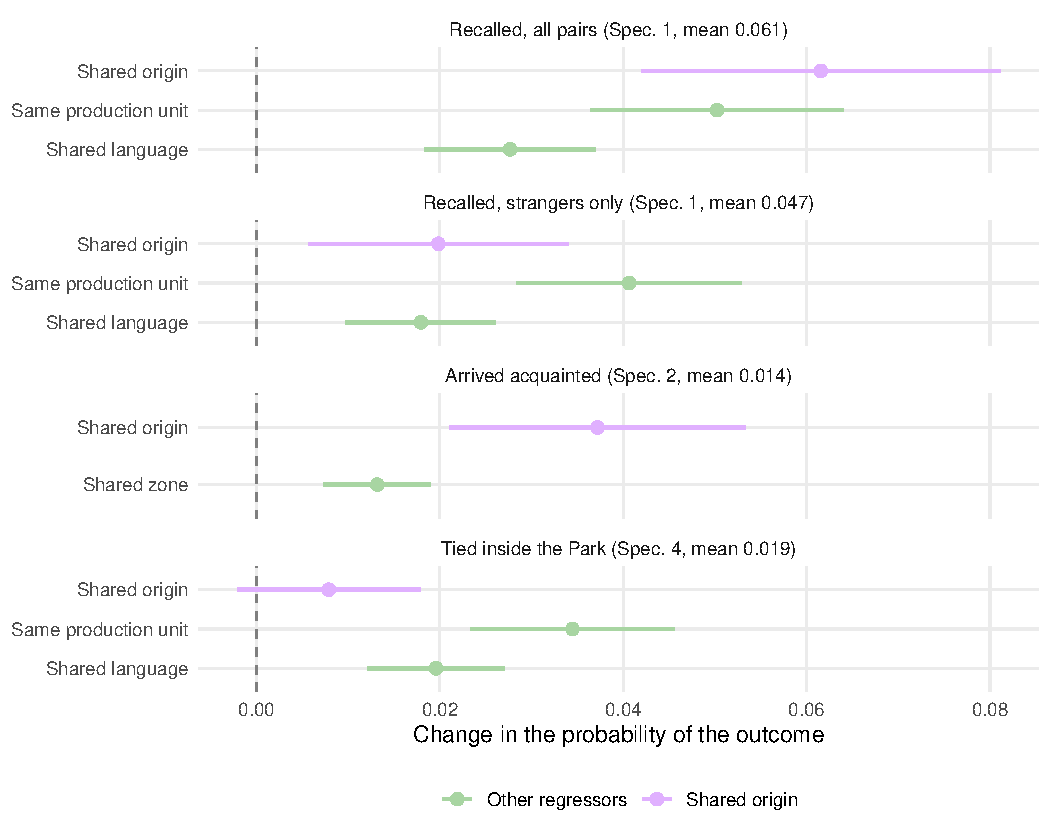
\includegraphics[width=0.85\textwidth]{../figures/fig_channels}
\fignote{Coefficients from Specification 1 on both of its samples, then Specifications 2 and 4, with 95\% confidence intervals. The four panels have different outcomes or samples, and different base rates, printed in each panel heading, but one common horizontal axis: the coefficients are all in probability points and rescaling each panel to its own base would make the panels incomparable, which is the comparison the figure exists to make.}
\end{figure}

\begin{table}[h!]
\centering
\caption{Specifications 2 to 4 - whether two workers are tied}
\label{tab:tie_formation}
\small% GENERATED by "21 analysis - channels.R" - do not edit by hand.
\begin{tabular}{lcccc}
& \shortstack{\textit{(2, inherited}\\\textit{ties)}} & \shortstack{\textit{(3, new ties)}} & \shortstack{\textit{(4, new ties,}\\\textit{same woreda)}} & \shortstack{\textit{(4, new ties,}\\\textit{same zone)}} \\
\dmidrule
Shared origin & 0.037*** & --- & 0.008 & --- \\
 & (0.008) &  & (0.005) &  \\
Shared zone & 0.013*** & --- & --- & 0.010*** \\
 & (0.003) &  &  & (0.003) \\
Same production unit & --- & 0.025*** & 0.034*** & 0.035*** \\
 &  & (0.004) & (0.006) & (0.006) \\
Shared language & --- & 0.011*** & 0.020*** & 0.018*** \\
 &  & (0.002) & (0.004) & (0.004) \\
\midrule
Sample & all pairs & strangers & strangers & strangers \\
Fixed effects & batch & batch & worker, alter & worker, alter \\
Observations & 19{,}522 & 19{,}239 & 19{,}239 & 19{,}239 \\
Mean of the outcome & 0.014 & 0.019 & 0.019 & 0.019 \\
MDE (80\% power) & --- & --- & 0.014 & 0.008 \\
\bottomrule
\end{tabular}

\fignote{Standard errors clustered on both members of the pair. *** 1\%, ** 5\%, * 10\%.}
\end{table}
\bigskip
\FloatBarrier

\noindent \underline{\textit{Specification 5: Exclusion}} \\[0.4em]
When considering a survey respondant of majority background, a minority is named \pnChanExclDeltaOutPp{} percentage points less often on the region definition ($\delta = \pnChanExclDeltaOut{}$, $p = \pnChanExclDeltaOutP{}$) and \pnChanExclLangDeltaOutPp{} points less often on the language definition ($\delta = \pnChanExclLangDeltaOut{}$, $p = \pnChanExclLangDeltaOutP{}$). Neither are powered nor significant. However, when the respondant is a minority worker herself, the penalty reverses into a significant premium of $\pnChanExclDeltaIn{}$ by region and $\pnChanExclLangDeltaIn{}$ by language (Table~\ref{tab:exclusion}). \\

\begin{table}[h!]
\centering
\caption{Specification 5 - whether a worker is refused}
\label{tab:exclusion}
\small% GENERATED by "21 analysis - channels.R" - do not edit by hand.
\begin{tabular}{lcc}
& \shortstack{\textit{(region)}} & \shortstack{\textit{(language)}} \\
\dmidrule
Receiver is minority & 0.005 & 0.005 \\
 & (0.004) & (0.004) \\
$\times$ namer is minority too & -0.031*** & -0.047*** \\
 & (0.010) & (0.013) \\
\midrule
Estimated on & dyads & dyads \\
Fixed effects & batch & batch \\
Observations & 19{,}522 & 19{,}522 \\
MDE (80\% power) & 0.010 & 0.011 \\
\bottomrule
\end{tabular}

\fignote{\textit{Region} defines minority as birth outside the Sidama region, \textit{language} as not speaking Sidamigna. Coefficients are $\delta$, so a positive number means the receiver is named \textit{less}. Standard errors clustered on both members of the pair. *** 1\%, ** 5\%, * 10\%.}
\end{table}
\bigskip


\clearpage
\parhead{Intensive margin}

\noindent \underline{\textit{Specification 6: Depth}} \\[0.4em]
\noindent Tie tenure is associated with deeper ties. Inherited co-hire ties carry \pnMuxDepthCohireInh{} layers on average, against \pnMuxDepthCohireNew{} for ties formed inside the Park (Table~\ref{tab:depth_cohire}). \\[-0.6em]

\noindent Shared origin does not deepen a tie. I get \pnMuxOriginCohire{} on the co-hire roster ($p = \pnMuxOriginCohireP{}$) and \pnMuxOriginGn{} in the general network ($p = \pnMuxOriginGnP{}$, Table~\ref{tab:depth_gn}). Both are negative and both are significant at the 5\% level or better. They also survive the kin and friend controls of column (3).  Interacting shared origin with vintage (tie inheritance) is not conclusive. \\[-0.6em]
 
 \noindent Thus, conditional on knowing someone at all, workers show no preference for their co-villagers. A shared woreda is associated with a narrower relationship rather than a richer one. What predicts the depth is whether they are related or friends to the alter. Kin and friends carry substantially more than acquaintances on the co-hire roster (\pnMuxKinCohire{} for kin), and somewhat less in the general network (\pnMuxKinGn{}).\\[-0.6em]
 
 \noindent Note that these estimates are limited by power\footnote{The co-hire column rests on \pnMuxOriginInhCellCohire{} same-woreda ties formed inside the Park. The vintage coefficient is identified only from workers reporting ties of both vintages (\pnMuxVintTiesCohire{} ties on the co-hire roster, \pnMuxVintTiesGn{} ties in the general network). Only \pnMuxPostCohire{} co-hire ties were formed after HIP, against \pnMuxPostGn{} general-network ones.}. Most workers are absorbed by the fixed effect and do not contribute to the estimate. \\

\begin{table}[h!]
\centering
\caption{Specification 6 - what makes a co-hire tie deep}
\label{tab:depth_cohire}
\small% GENERATED by "23 analysis - multiplexity.R" - do not edit by hand.
\begin{tabular}{lcccc}
& \shortstack{\textit{(6, no worker}\\\textit{FE)}} & \shortstack{\textit{(6, worker FE)}} & \shortstack{\textit{(6, + kin and}\\\textit{friend)}} & \shortstack{\textit{(6, +}\\\textit{origin~$\times$~vintage)}} \\
\dmidrule
Tie predates HIP & 0.41*** & 0.80*** & 0.61*** & 0.63*** \\
 & (0.06) & (0.17) & (0.18) & (0.18) \\
Shared birth woreda & -0.02 & -0.53** & -0.48* & -0.04 \\
 & (0.09) & (0.23) & (0.25) & (0.27) \\
Same woreda $\times$ pre-HIP & --- & --- & --- & -0.55 \\
 &  &  &  & (0.36) \\
Shared language & 0.05 & 1.03* & 0.81 & 0.82 \\
 & (0.15) & (0.53) & (0.51) & (0.51) \\
Same production unit & -0.06 & 0.14 & 0.16 & 0.16 \\
 & (0.06) & (0.17) & (0.16) & (0.16) \\
Kin & --- & --- & 0.86*** & 0.91*** \\
 &  &  & (0.29) & (0.28) \\
Friends & --- & --- & 0.84*** & 0.86*** \\
 &  &  & (0.16) & (0.15) \\
\midrule
Worker fixed effects & no & yes & yes & yes \\
Ties & 476 & 249 & 249 & 249 \\
Workers & --- & 117 & 117 & 117 \\
\bottomrule
\end{tabular}

\fignote{Standard errors clustered on both members of the pair. *** 1\%, ** 5\%, * 10\%.}
\end{table}
\clearpage

\noindent \underline{\textit{Specification 7: Vintage}} \\[0.4em]
\noindent  The  most common tie in the roster (workplace break, \pnMuxBreaksPrevCohire{}\% of ties) is not more likely to be associated with inherited ties. As expected, being a general network member is negatively associated with workplace ties. An alter known before HIP is markedly less likely to be someone the worker takes breaks with (\pnMuxBreaksGn{}), and more likely to be someone she would turn to for a large expense (\pnMuxLargeExpGn{}). This is consistent with the general network being at the village of origin (Table~\ref{tab:vintage_layers}, Figure~\ref{fig:layer_vintage}).

\begin{table}[h!]
\centering
\caption{Specification 7 - which layers an inherited tie carries}
\label{tab:vintage_layers}
\small% GENERATED by "23 analysis - multiplexity.R" - do not edit by hand.
\begin{tabular}{lcc}
\textit{layer} & \shortstack{\textit{(7, co-hire ties)}} & \shortstack{\textit{(7, general network)}} \\
\dmidrule
rosca ekub & 0.031 (0.038) & 0.021 (0.018) \\
assistance (out) & 0.037 (0.038) & 0.106*** (0.025) \\
large expenses (out) & 0.040 (0.028) & 0.099*** (0.021) \\
borrow money (out) & 0.060 (0.074) & 0.065** (0.031) \\
large expenses (in) & 0.077 (0.059) & 0.309*** (0.023) \\
call or text & 0.094 (0.084) & 0.162*** (0.035) \\
friends & 0.097 (0.111) & 0.058 (0.039) \\
workplace breaks & 0.105 (0.087) & -0.505*** (0.042) \\
meet outside work & 0.173* (0.091) & 0.085** (0.037) \\
job search & 0.188** (0.086) & 0.120*** (0.029) \\
borrow money (in) & 0.210** (0.087) & 0.063* (0.037) \\
assistance (in) & 0.213*** (0.061) & 0.187*** (0.031) \\
advice personal decision & 0.250*** (0.094) & 0.151*** (0.028) \\
navigate hawassa & 0.301*** (0.083) & 0.126*** (0.030) \\
commute & 0.321*** (0.083) & -0.130*** (0.040) \\
\midrule
Ties & 399 & 3{,}029 \\
\bottomrule
\end{tabular}

\end{table}

\begin{figure}[h!]
\centering
\caption{Specification 7 - which layers an inherited tie carries}
\label{fig:layer_vintage}
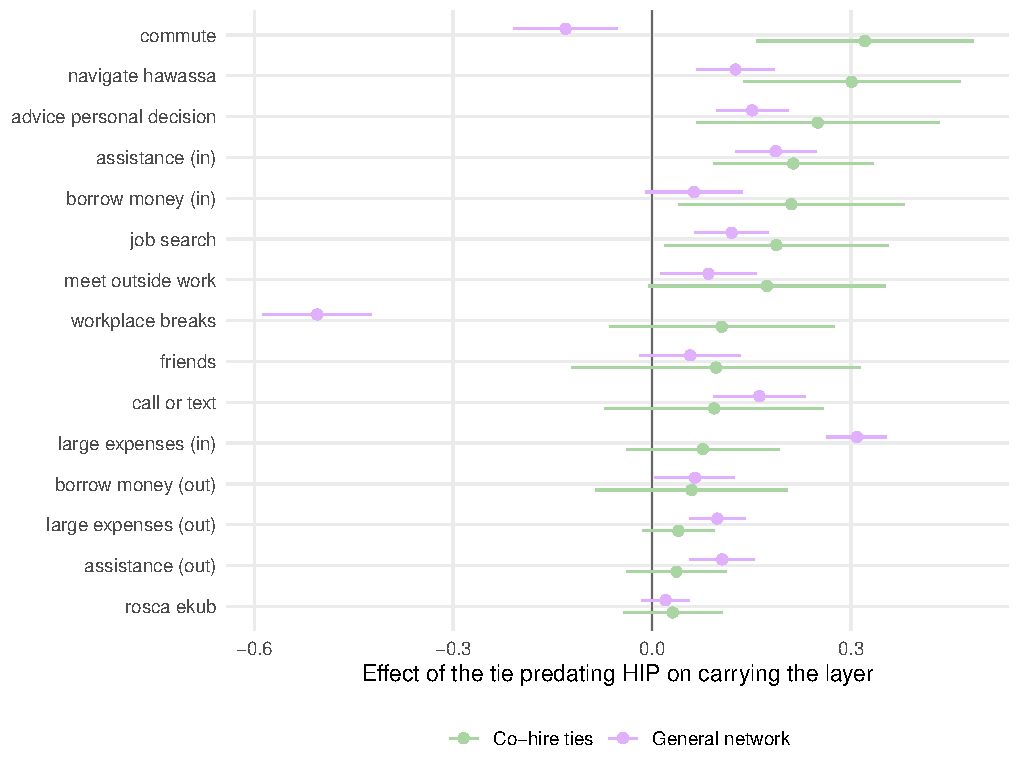
\includegraphics[width=0.7\textwidth]{../figures/fig_layer_vintage}
\end{figure}
\clearpage

\noindent \underline{\textit{Specification 8: Multiplexing}} \\

\noindent Specification 6 said a co-villager tie is not deeper. This one asks whether it is differently shaped (\textit{i.e.} if it loads on different functions), and it appears to be.\\[-0.6em]

\noindent In the general network, ties tilted toward money and help and away from company (Table~\ref{tab:layers_gn}). A same-woreda tie is more likely to be someone the worker would turn to for a large expense (\pnLayerLargeExpGn{}) and less likely to be someone she takes her workplace breaks with (\pnLayerBreaksGn{}), these consistent with the general network being away from HIP.\\[-0.6em]

\noindent Origin here masks kin - \pnLayerKinShareGn{}\% of the \pnLayerOriginTiesGn{} same-origin ties are kin, against \pnLayerKinShareGnNon{}\% of the rest. Fitted side by side the origin profile and the kinship profile trace nearly the same shape across the fifteen layers (correlation \pnLayerProfileCorrGn{}). 

\noindent Holding kinship, vintage and co-residence fixed , the money layers disappear. Two co-villagers who are not relatives are less likely to be workplace company, whether taking breaks (\pnLayerBreaksGnCtrl{}) or finding one's way around Hawassa (\pnLayerNavigateGnCtrl{}, the one coefficient the controls barely move), but more likely to be named friends (\pnLayerFriendsGnCtrl{}, against \pnLayerFriendsGn{} before). I read this as the co-villager relation being an affective one rather than a practical one, once the family tie is taken out (Figure~\ref{fig:layer_origin}). \\[-0.6em]

\noindent The co-hire roster shows no comparable reshaping, but with only \pnLayerOriginTiesCohire{} of \pnLayerTiesCohire{} co-hire ties sharing a woreda this is an underpowered null (Table~\ref{tab:layers_cohire}). \\[-0.6em]
\bigskip

\begin{table}[h!]
\centering
\caption{Specification 8 - what a shared origin does to what a general-network tie is for}
\label{tab:layers_gn}
\small% GENERATED by "22 analysis - layer design.R" - do not edit by hand.
\begin{tabular}{lcc}
\textit{layer} & \shortstack{\textit{(8, no controls)}} & \shortstack{\textit{(8, + kinship, vintage, co-residence)}} \\
\dmidrule
advice personal decision & 0.034** (0.014) & -0.005 (0.016) \\
borrow money (in) & 0.010 (0.015) & 0.012 (0.017) \\
large expenses (in) & 0.203*** (0.015) & 0.017 (0.016) \\
job search & 0.001 (0.014) & -0.007 (0.016) \\
navigate hawassa & -0.042*** (0.014) & -0.047*** (0.015) \\
commute & -0.066*** (0.015) & 0.003 (0.018) \\
meet outside work & -0.058*** (0.015) & 0.008 (0.017) \\
call or text & 0.027* (0.015) & 0.026 (0.017) \\
workplace breaks & -0.147*** (0.016) & -0.055*** (0.017) \\
friends & -0.061*** (0.016) & 0.052*** (0.018) \\
assistance (in) & 0.081*** (0.014) & 0.004 (0.015) \\
rosca ekub & -0.015 (0.011) & 0.001 (0.012) \\
borrow money (out) & -0.035*** (0.013) & -0.002 (0.014) \\
large expenses (out) & 0.070*** (0.011) & 0.004 (0.012) \\
assistance (out) & -0.001 (0.011) & -0.010 (0.012) \\
\midrule
Joint test, $\chi^2(14)$ & 286.63*** & 33.33*** \\
Ties & 3{,}030 & 3{,}030 \\
\hspace{1em}of which shared origin & 1{,}952 & 1{,}952 \\
Tie-by-layer observations & 45{,}450 & 45{,}450 \\
\bottomrule
\end{tabular}

\fignote{Standard errors clustered on the pair. *** 1\%, ** 5\%, * 10\%.}
\end{table}

\begin{table}[h!]
\centering
\caption{Specification 8 - what a shared origin does to what a co-hire tie is for}
\label{tab:layers_cohire}
\small% GENERATED by "22 analysis - layer design.R" - do not edit by hand.
\begin{tabular}{lcc}
\textit{layer} & \shortstack{\textit{(8, no controls)}} & \shortstack{\textit{(8, + kinship, vintage, co-residence)}} \\
\dmidrule
advice personal decision & 0.046 (0.044) & 0.042 (0.047) \\
borrow money (in) & 0.050 (0.048) & 0.009 (0.050) \\
large expenses (in) & -0.023 (0.031) & -0.008 (0.033) \\
job search & 0.003 (0.049) & 0.023 (0.052) \\
navigate hawassa & -0.001 (0.047) & -0.044 (0.047) \\
commute & 0.047 (0.047) & -0.003 (0.049) \\
meet outside work & 0.123** (0.048) & 0.058 (0.049) \\
call or text & -0.076 (0.048) & -0.092* (0.051) \\
workplace breaks & 0.002 (0.050) & 0.044 (0.053) \\
friends & -0.014 (0.050) & 0.022 (0.051) \\
assistance (in) & -0.023 (0.038) & -0.018 (0.039) \\
rosca ekub & -0.019 (0.031) & 0.025 (0.033) \\
borrow money (out) & -0.038 (0.037) & -0.026 (0.040) \\
large expenses (out) & -0.024 (0.027) & 0.003 (0.025) \\
assistance (out) & -0.052** (0.023) & -0.034 (0.026) \\
\midrule
Joint test, $\chi^2(14)$ & 18.31 & 14.28 \\
Ties & 652 & 652 \\
\hspace{1em}of which shared origin & 90 & 90 \\
Tie-by-layer observations & 9{,}780 & 9{,}780 \\
\bottomrule
\end{tabular}

\fignote{Standard errors clustered on the pair. *** 1\%, ** 5\%, * 10\%.}
\end{table}

\FloatBarrier

\begin{figure}[h!]
\centering
\caption{Shared origin, and what survives holding kinship fixed}
\label{fig:layer_origin}
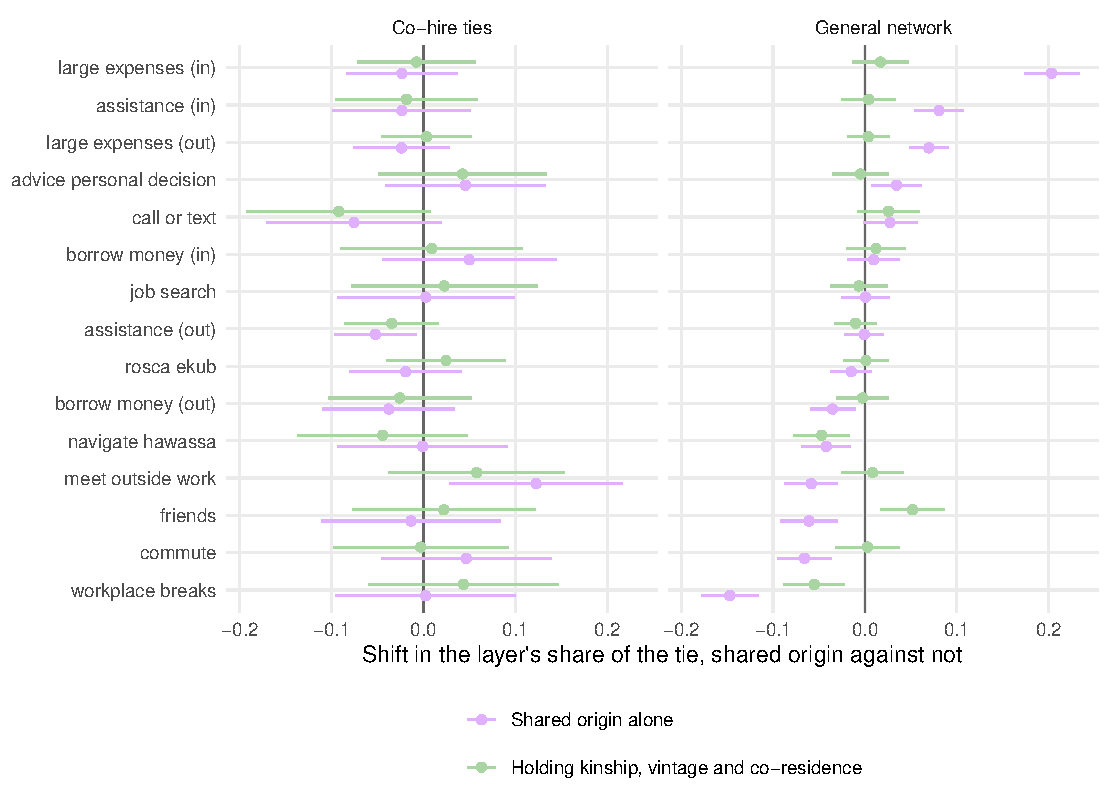
\includegraphics[width=0.95\textwidth]{../figures/fig_layer_origin}
\end{figure}
\clearpage


\clearpage
\section{Conclusions}
\label{sec:conclusion}
\noindent I set out to ask which mechanism produces homophily in the networks of newcomers. The short answer is that  the same-origin composition of these workers' networks is inherited rather than produced inside the Park. This is expected given the nature of my data, as we see the beginning of network formation (and nothing else). Within HIP, from what we can see, ties seem to depend on prolonged exposure from sharing a unit and whether the worker can be understood. \\


\noindent \textit{Importation.} This is the channel that carries the same-origin premium. Two workers from the same woreda are \pnChanImportOriginRel{} times as likely as any other pair to have arrived already acquainted. The premium is hyperlocal, \textit{i.e.} depends on woreda ties rather than zones. A shared woreda raises the chance that a worker produces a co-hire's name at all, but once the pairs she arrived knowing are set aside, that premium falls to the low end of the bracket reported in Section~\ref{sec:results}. \\

\noindent \textit{Opportunity.} Among the pairs who arrived as strangers, the firm's having placed the two in the same production unit multiplies the chance of a tie by \pnChanOppUnitRel{}. Two workers who cannot converse form a tie at \pnChanOppKappa{} of the rate of two who can. Both are estimated on pairs who met for the first time at HIP. \\

\noindent \textit{Taste.} At the woreda level I find nothing, and it is probably because I cannot detect it. The point estimate is \pnChanTasteTauPp{} of a percentage point, but the smallest effect this design would catch is \pnChanTasteMdePp{} percentage points (calculating the minimum detectable effect), which is the base tie rate itself. I can however rule out a big taste effect. On depth, shared origin does not make a tie deeper — it makes it slightly thinner, significantly so on both rosters once the worker is held fixed (\pnMuxOriginCohire{} on the co-hire side, \pnMuxOriginGn{} in the general network). Holding the layer profiles of kinship, vintage and co-residence, most of what origin predicts about tie content disappears. \\

\noindent \textit{Exclusion.} Among majority respondant the penalty insignificant. Minority workers name each other markedly more. This is also underpowered.

\noindent  If these results held with a better identification strategy and possibly a panel, this may imply that the institution has actually a big impact on how homophilous the newcomers' network can be. How it recruits and how it assigns production units can shape these people's networks. \\

\parhead{Limitations}

\noindent The first limitation is that this is a single cross-section, taken once, a median of \pnHireLagMedian{} days after the workers were hired. A panel would replace the whole construction, as I could observe the evolutions of ties, and assess if kinship becomes less prevalent over time. From my understanding, kin represents the key social and insurance institution in Ethiopia, so this would be a very important aspect to study. \\

\noindent The second limitation is power, and it falls on the two channels I do not detect. Taste rests on \pnChanTasteOriginPairs{} same-woreda pairs who arrived as strangers, of whom \pnChanTasteTies{} went on to be tied. Exclusion rests on the pairs in which exactly one of the two is a minority worker, \pnChanExclOutPairs{} of them. Nulls estimated on that much variation are not evidence of absence and are not reported as such anywhere in this thesis. \\



\newpage
\bibliographystyle{apalike}
\bibliography{../sources}
\newpage
\appendix
% appendix floats numbered A1, A2, ... so cross-references from the body are
% unambiguous about which are relegated here
\renewcommand{\thefigure}{A\arabic{figure}}
\setcounter{figure}{0}
\renewcommand{\thetable}{A\arabic{table}}
\setcounter{table}{0}

\clearpage
\section{Additional figures}
\label{sec:appendix}

\begin{table}[h!]
\centering
\caption{Firms in the analysis sample}
\label{tab:firms}
% GENERATED by "13 descriptives - sample and firms.R" - do not edit by hand.
\begin{tabular}{lrrrrr}
\textit{firm} & \textit{rostered} & \textit{surveyed} & \textit{share of sample} & \textit{sampling rate} & \textit{co-hire sets} \\
\dmidrule
Firm B & 326 & 269 & 0.40 & 0.82 & 15 \\
Firm A & 396 & 255 & 0.38 & 0.64 & 21 \\
Firm C & 251 & 97 & 0.14 & 0.39 & 18 \\
Firm E & 113 & 38 & 0.06 & 0.34 & 8 \\
Firm F & 25 & 10 & 0.01 & 0.40 & 3 \\
\midrule
Total & 1{,}111 & 669 & & & 65 \\
\bottomrule
\end{tabular}

\fignote{\textit{sampling rate} is \textit{surveyed} over \textit{rostered}. \textit{Co-hire sets} counts the distinct hiring batches with at least one surveyed member.}
\end{table}

\begin{table}[h!]
\centering
\caption{Sample characteristics}
\label{tab:demographics}
\small% GENERATED by "13 descriptives - sample and firms.R" - do not edit by hand.
\begin{tabular}{lrrrrrr}
& \multicolumn{2}{c}{\textit{all}} & \multicolumn{2}{c}{\textit{majority-rural}} & \multicolumn{2}{c}{\textit{urban background}} \\
\cmidrule(lr){2-3}\cmidrule(lr){4-5}\cmidrule(lr){6-7}
& \textit{mean} & \textit{sd} & \textit{mean} & \textit{sd} & \textit{mean} & \textit{sd} \\
\dmidrule
Age & 23.51 & 2.91 & 23.40 & 2.74 & 24.14 & 3.67 \\
Female & 0.92 & 0.27 & 0.93 & 0.26 & 0.86 & 0.35 \\
Education (1-12) & 6.72 & 2.86 & 6.75 & 2.84 & 6.56 & 2.96 \\
Completed grade 10 & 0.94 & 0.23 & 0.95 & 0.22 & 0.90 & 0.30 \\
Married & 0.21 & 0.41 & 0.19 & 0.40 & 0.29 & 0.46 \\
Has children & 0.02 & 0.14 & 0.02 & 0.14 & 0.03 & 0.16 \\
Household size & 1.72 & 1.15 & 1.60 & 0.98 & 2.40 & 1.67 \\
Born in Sidama & 0.85 & 0.35 & 0.87 & 0.34 & 0.78 & 0.41 \\
Speaks Sidamigna (1-5) & 4.24 & 1.30 & 4.34 & 1.22 & 3.72 & 1.61 \\
Speaks Amharic (1-5) & 2.98 & 0.97 & 2.84 & 0.88 & 3.75 & 1.06 \\
Share of life urban & 0.32 & 0.27 & 0.22 & 0.12 & 0.88 & 0.18 \\
Years in Hawassa & 6.51 & 6.12 & 4.59 & 2.81 & 17.27 & 8.16 \\
Co-hire set size & 39.20 & 23.32 & 39.71 & 23.56 & 36.36 & 21.78 \\
Days since hire & 41.02 & 28.06 & 41.46 & 28.42 & 38.49 & 25.93 \\
\midrule
Workers & \multicolumn{2}{c}{672} & \multicolumn{2}{c}{570} & \multicolumn{2}{c}{102} \\
\bottomrule
\end{tabular}

\fignote{\textit{majority-rural}: more than half of life spent rural.}
\end{table}
\clearpage

\begin{table}[h!]
\centering
\caption{Livelihoods}
\label{tab:livelihoods}
\small% GENERATED by "15 descriptives - livelihoods.R" - do not edit by hand.
\begin{tabular}{llrrrrr}
& & \textit{n} & \textit{p25} & \textit{median} & \textit{p75} & \textit{p90} \\
\dmidrule
Monthly wage at HIP & Birr & 670 & 2500.0 & 2500.0 & 3200.0 & 4000.0 \\
Own earnings, all activities & Birr/month & 511 & 2498.6 & 2785.7 & 3428.6 & 4285.7 \\
Household income, past 3 months & Birr & 672 & 11745.0 & 16801.5 & 24000.0 & 32140.0 \\
Rent & Birr/month & 672 & 500.0 & 750.0 & 1000.0 & 1250.0 \\
Rent as a share of own earnings & ratio & 475 & 0.2 & 0.2 & 0.3 & 0.5 \\
Expected wage in one year & Birr & 654 & 3000.0 & 4000.0 & 5000.0 & 6000.0 \\
Reservation wage, outside offer & Birr & 606 & 5000.0 & 6000.0 & 8000.0 & 10000.0 \\
Reservation wage / current wage & ratio & 606 & 1.6 & 2.0 & 2.8 & 4.0 \\
Days spent finding this job & days & 672 & 10.0 & 20.0 & 30.0 & 60.0 \\
\bottomrule
\end{tabular}

\fignote{\textit{Own earnings, all activities} is the fourteen-day earnings module scaled to a month, for the \pnEarnWindowN{} workers whose window falls entirely after their hire date.}
\end{table}

% GENERATED by "12 descriptives - batch composition.R" - do not edit by hand.
\begin{table}[h!]
\centering
\caption{Survey coverage of the hiring batches}
\label{tab:coverage}
\begin{tabular}{lrrrrrr}
\textit{batch} & \textit{firm} & \textit{size} & \textit{line} & \textit{interviewed} & \textit{typed} & \textit{coverage} \\
\dmidrule
batch\_20 & Firm B & 17 & yes & 17 & 16 & 0.94 \\
batch\_05 & Firm A & 55 & -- & 51 & 51 & 0.93 \\
batch\_16 & Firm A & 39 & -- & 37 & 36 & 0.92 \\
batch\_19 & Firm A & 36 & -- & 34 & 33 & 0.92 \\
batch\_42 & Firm A & 45 & -- & 41 & 41 & 0.91 \\
batch\_29 & Firm A & 91 & -- & 82 & 81 & 0.89 \\
batch\_02 & Firm A & 73 & -- & 66 & 65 & 0.89 \\
batch\_62 & Firm A & 18 & -- & 16 & 16 & 0.89 \\
\midrule
\multicolumn{7}{c}{\textit{36 further batches omitted}} \\
\midrule
batch\_48 & Firm C & 27 & -- & 6 & 6 & 0.22 \\
batch\_49 & Firm C & 27 & -- & 6 & 6 & 0.22 \\
batch\_50 & Firm C & 27 & -- & 6 & 6 & 0.22 \\
batch\_51 & Firm C & 27 & -- & 6 & 6 & 0.22 \\
batch\_52 & Firm C & 27 & -- & 6 & 6 & 0.22 \\
batch\_54 & Firm C & 27 & -- & 6 & 6 & 0.22 \\
batch\_11 & Firm C & 27 & yes & 5 & 5 & 0.19 \\
batch\_53 & Firm C & 27 & -- & 6 & 5 & 0.19 \\
\bottomrule
\end{tabular}
\fignote{One row is a hiring batch with at least 10 rostered workers (13 smaller batches omitted), ordered by \textit{coverage}, the share of the roster that entered the analysis sample: the 8 best and 8 worst are shown, 36 omitted between. \textit{line} marks a closed hiring line; \textit{typed} counts interviewed workers with a recorded birthplace.}
\end{table}


\begin{table}[h!]
\centering
\caption{Specification 6 - what makes a general-network tie deep}
\label{tab:depth_gn}
\small% GENERATED by "23 analysis - multiplexity.R" - do not edit by hand.
\begin{tabular}{lcccc}
& \shortstack{\textit{(6, no worker}\\\textit{FE)}} & \shortstack{\textit{(6, worker FE)}} & \shortstack{\textit{(6, + kin and}\\\textit{friend)}} & \shortstack{\textit{(6, +}\\\textit{origin~$\times$~vintage)}} \\
\dmidrule
Tie predates HIP & 0.20*** & 0.32*** & 0.33*** & 0.34*** \\
 & (0.06) & (0.07) & (0.07) & (0.09) \\
Alter from same woreda & -0.12*** & -0.12*** & -0.07* & -0.04 \\
 & (0.03) & (0.04) & (0.04) & (0.14) \\
Same woreda $\times$ pre-HIP & --- & --- & --- & -0.03 \\
 &  &  &  & (0.15) \\
Living together & 0.36*** & 0.37*** & 0.40*** & 0.40*** \\
 & (0.04) & (0.04) & (0.04) & (0.04) \\
Kin & --- & --- & 0.45*** & 0.45*** \\
 &  &  & (0.08) & (0.08) \\
Friends & --- & --- & 0.68*** & 0.68*** \\
 &  &  & (0.08) & (0.08) \\
\midrule
Worker fixed effects & no & yes & yes & yes \\
Ties & 3{,}030 & 3{,}022 & 3{,}022 & 3{,}022 \\
Workers & --- & 661 & 661 & 661 \\
\bottomrule
\end{tabular}

\fignote{Standard errors clustered on the respondent. *** 1\%, ** 5\%, * 10\%.}
\end{table}
\clearpage

% GENERATED by "21 analysis - channels.R" - do not edit by hand.
\begin{table}[h!]
\centering
\caption{Does the functional form matter? Linear against logit}
\label{tab:logit}
\begin{tabular}{lcc}
\textit{equation and regressor} & \textit{LPM} & \textit{logit} \\
\dmidrule
\textit{Specification 1, recall} & 19{,}522 & 19{,}383 \\
\quad Shared origin & 6.15*** & 4.51*** \\
\quad Same production unit & 5.02*** & 5.05*** \\
\quad Production unit recorded & -0.75 & -0.83 \\
\quad Shared language & 2.77*** & 3.73*** \\
\midrule
\textit{Specification 2, inherited ties} & 19{,}522 & 18{,}897 \\
\quad Shared origin & 3.72*** & 1.34*** \\
\quad Shared zone & 1.32*** & 1.28*** \\
\midrule
\textit{Specification 3, new ties} & 19{,}239 & 18{,}875 \\
\quad Same production unit & 2.47*** & 2.53*** \\
\quad Production unit recorded & -0.07 & -0.21 \\
\quad Shared language & 1.12*** & 1.71*** \\
\midrule
\textit{Specification 4, new ties} & 19{,}239 & 18{,}875 \\
\quad Shared origin & 0.45 & 0.46 \\
\quad Same production unit & 2.47*** & 2.54*** \\
\quad Production unit recorded & -0.07 & -0.22 \\
\quad Shared language & 1.10*** & 1.69*** \\
\bottomrule
\end{tabular}
\fignote{Entries are percentage points. Stars mark 10, 5 and 1 percent.}
\end{table}

\clearpage

\begin{figure}[h!]
\centering
\caption{Birth woreda of sampled workers}
\label{fig:catchment}
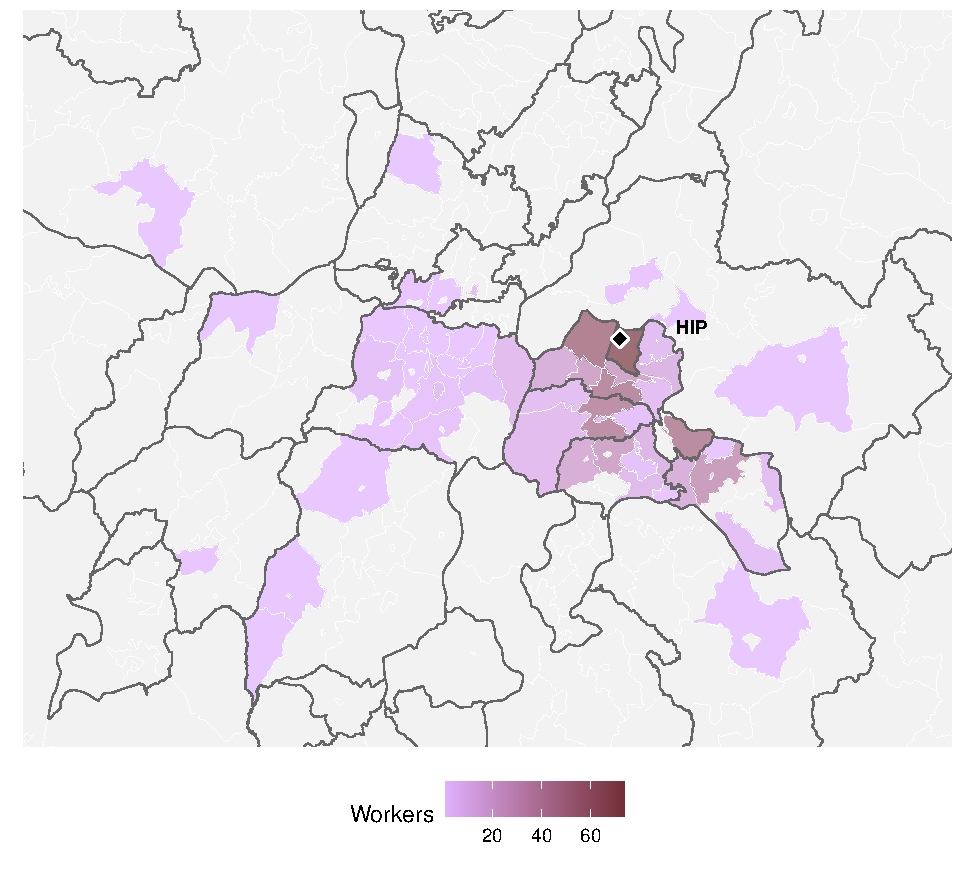
\includegraphics[width=0.7\textwidth]{../figures/fig_setting_catchment}
\fignote{Map extent is limited to Southern Ethiopia.}
\end{figure}

\begin{figure}[h!]
\centering
\caption{Size of the co-hire group}
\label{fig:cohires}
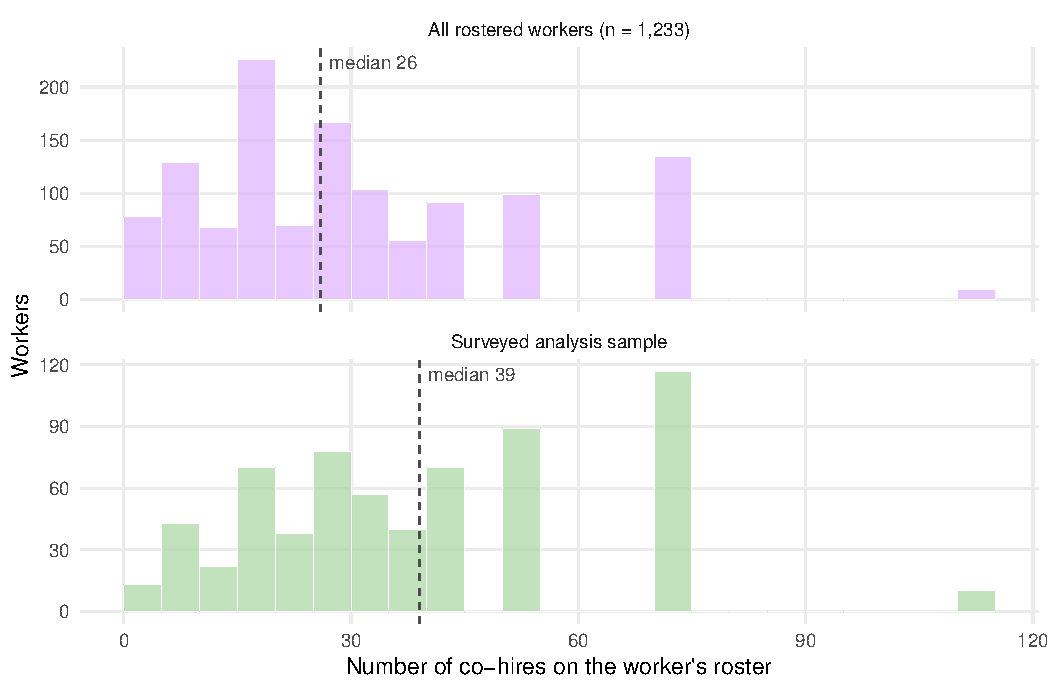
\includegraphics[width=0.7\textwidth]{../figures/fig_setting_cohires}
\fignote{Top panel: all rostered workers. Bottom panel: the surveyed analysis sample.}
\end{figure}

\begin{figure}[h!]
\centering
\caption{Co-residents by type and rural background}
\label{fig:housing}
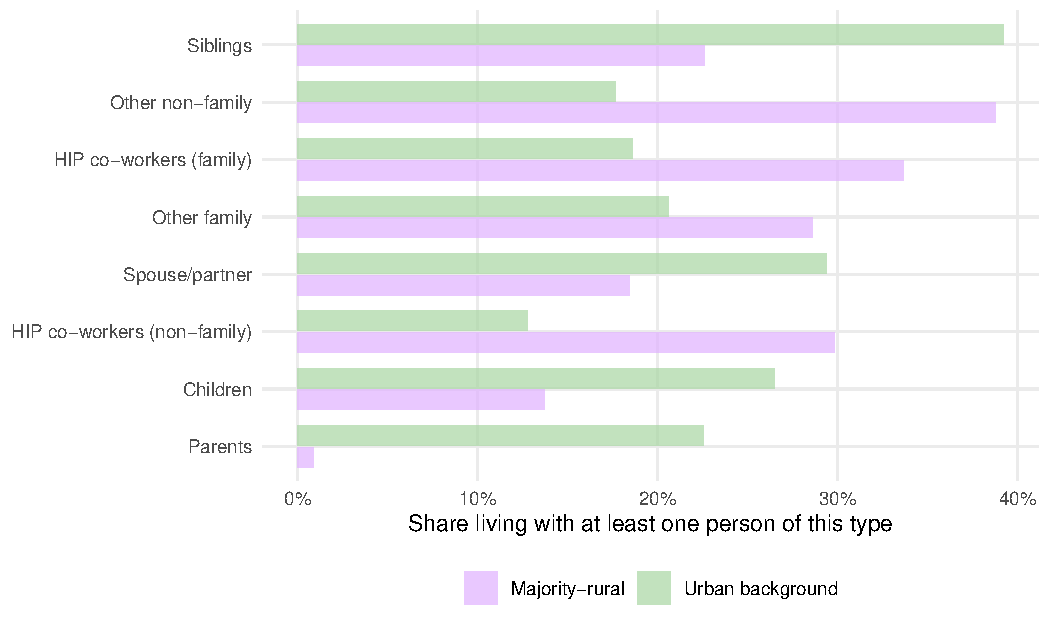
\includegraphics[width=0.9\textwidth]{../figures/fig_setting_housing}
\fignote{Bars show the share of workers living with at least one person of each type.}
\end{figure}

\begin{figure}[h!]
\centering
\caption{Generator coverage over the co-hire roster}
\label{fig:generators}
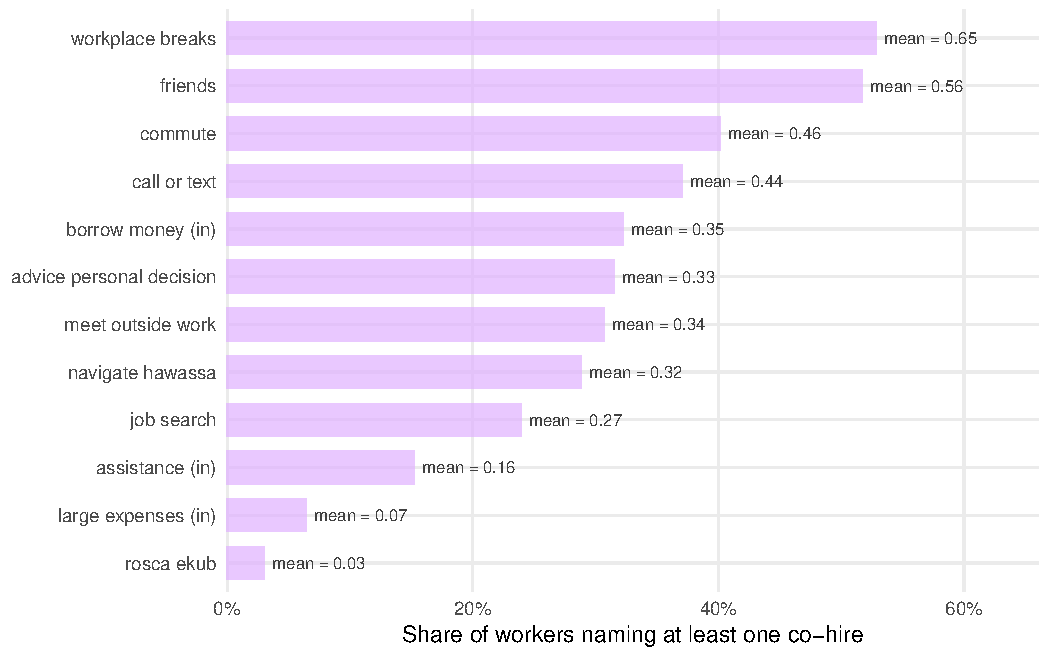
\includegraphics[width=0.9\textwidth]{../figures/fig_setting_generators}
\fignote{Share of workers naming at least one co-hire under each generator.}
\end{figure}

\clearpage
\section{Tests}
\label{sec:appendix-quasirandom}
\noindent This appendix explains and reports the tests mentioned in Section~\ref{sec:strategy}.\\

\noindent Recall that workers are hired in groups and undergo training together. Firms may have slightly different training protocols, but trainings usually last about two weeks and comprise both soft-skills and machine training. Following the training, workers are assigned to a production unit according to how well they have performed. The training group is assigned by recruitment and is not chosen by the workers. Training group sizes vary widely (Appendix Figure~\ref{fig:cohires}). I refer to a training group as a "batch", and I take a batch to be the set of workers whose preloaded hiring rows list an identical set of co-hires. There are \pnBatchesWord{} batches that contain at least one surveyed worker, of which \pnBatchesLine{} are closed hiring lines in the sense that every member names the same set of colleagues, the rest appear to be slices of some sort of rolling recruitment window. As mentioned earlier, I do not have detailed information on each member of the batch - on origin, for example, I have information on those who were interviewed and on the colleagues they mentioned as a tie. Coverage (\textit{i.e.} the portion of a batch that we have surveyed) varies, from \pnCoverageMaxPct{}\% to less than \pnCoverageMinPct{}\% (Appendix Table~\ref{tab:coverage}). \\

\noindent Even if workers do not choose their batch-mates, but probably get hired with the people who immigrated with them. The origin composition of a batch might serve as exogenous variation, but it must be tested. I try to test for it in different ways. \\

\parhead{Test 1 - urbanity prediction}

\noindent I test whether the "urbanity" of co-hires (\textit{i.e.}, how urban are the co-hires on average) predicts the profile of the worker herself. \\

\noindent For worker $i$ with characteristic $y_i$,
\begin{equation}
\label{eq:setting-balance}
y_i \;=\; a \;+\; \beta \, \bar{x}_{-i} \;+\; \varepsilon_i ,
\end{equation}
where $\bar{x}_{-i}$ is the mean share of life spent in an urban area among the members of $i$'s own co-hire set, excluding herself\footnote{I cannot use the share of urban individuals as it is extremely low and the exercise would lose its meaning. Additionally, I must leave out $i$, since counting the worker in her own treatment would lead to endogeneity. Excluding her is not neutral either, because she is drawn from the pool of co-hires}. Across workers $\bar{x}_{-i}$ has mean \pnTreatMean{} and standard deviation \pnTreatSd{}. The IQR stands between \pnTreatPTwentyFive{} and \pnTreatPSeventyFive{}. \\


\noindent If assignment was as good as random, then we would have $\beta=0$ for every characteristic. This implies the colleagues one is dealt should carry no information about oneself. I run \pnBalanceChars{} such regressions, one per row of Table~\ref{tab:balance}, with standard errors clustered on the batch, and a second specification adding a firm fixed effect so that where a firm recruits cannot pass as batch composition. Note that Table~\ref{tab:balance} reports the effect of a full unit of $\bar{x}_{-i}$, which no worker in this sample experiences. Moving from the first quartile of co-hire urbanity to the third is a change of \pnTreatPSeventyFive{}$-$\pnTreatPTwentyFive{}. \\

\noindent According to this test, no characteristic is predicted by batch composition.

% GENERATED by "20 analysis - balance.R" - do not edit by hand.
\begin{table}[h!]
\centering
\caption{Balance of worker characteristics on co-hire composition}
\label{tab:balance}
\begin{tabular}{lrrrrr}
\textit{outcome} & \textit{mean} & \textit{coef.} & \textit{s.e.} & \textit{$p$} & \textit{$p_{\text{ri}}$} \\
\dmidrule
Age & 23.51 & 2.304 & (1.682) & 0.18 & 0.117 \\
Female & 0.93 & 0.089 & (0.302) & 0.77 & 0.617 \\
Education (1--12) & 6.70 & 1.514 & (1.609) & 0.35 & 0.325 \\
Grade 10 or above & 0.94 & 0.068 & (0.080) & 0.40 & 0.444 \\
Married & 0.21 & 0.226 & (0.158) & 0.16 & 0.165 \\
Has children & 0.02 & 0.012 & (0.038) & 0.76 & 0.801 \\
Household size & 1.73 & 0.337 & (0.557) & 0.55 & 0.530 \\
Born in Sidama & 0.86 & -0.175 & (0.213) & 0.42 & 0.405 \\
Born in modal woreda & 0.09 & 0.070 & (0.190) & 0.71 & 0.667 \\
Sidamigna fluency (1--5) & 4.26 & -0.577 & (0.766) & 0.45 & 0.474 \\
Amharic fluency (1--5) & 2.97 & 0.350 & (0.718) & 0.63 & 0.503 \\
Share of life urban & 0.31 & 0.208 & (0.139) & 0.14 & 0.075 \\
Never lived rural & 0.09 & 0.154 & (0.165) & 0.35 & 0.169 \\
\bottomrule
\end{tabular}
\fignote{One row per characteristic: a regression of it on mean co-hire urbanity (share of life urban, worker excluded). 13 characteristics, 644 workers, 65 batches; s.e. clustered on batch. Stars mark 10, 5 and 1 percent. $p_{\text{ri}}$ is a randomisation-inference $p$-value from 2000 batch-level reassignments.}
\end{table}

\FloatBarrier

\parhead{Test 2 - batch prediction, not considering firms' catchments}

\noindent This tests whether the batch a worker was hired into tells me anything about her. I perform an $F$-test. The spread of any characteristic across the sample comes from two places. Workers in the same batch differ from one another, and batch averages differ from one another. If recruitment dealt workers out at random, batch averages should be around the overall average. The $F$ statistic is the ratio of the two. Near one, the batches look like random draws from a common pool. \\

\noindent The regression looks as follow. Writing $b(i)$ for the batch worker $i$ belongs to and $B$ for the number of batches,
\begin{equation}
\label{eq:setting-omnibus}
y_i \;=\; \sum_{b=1}^{B} \bar{y}_b \, \mathds{1}\{b(i)=b\} \;+\; \varepsilon_i ,
\qquad
H_0 : \; \bar{y}_1 = \bar{y}_2 = \cdots = \bar{y}_B .
\end{equation}
The coefficient on each dummy is that batch's own mean of the characteristic, so the null is that the batch means are all equal. \\

% GENERATED by "20 analysis - balance.R" - do not edit by hand.
\begin{table}[h!]
\centering
\caption{Is a characteristic predicted by batch membership?}
\label{tab:omnibus}
\begin{tabular}{lrrr}
\textit{characteristic} & \textit{F} & \textit{$p$} & \textit{$p_{\text{ri}}$} \\
\dmidrule
Age & 1.50 & 0.010 & 0.033 \\
Female & 10.63 & $<$0.001 & 0.000 \\
Education (1--12) & 1.87 & $<$0.001 & 0.000 \\
Grade 10 or above & 1.41 & 0.023 & 0.134 \\
Married & 1.30 & 0.064 & 0.059 \\
Has children & 0.24 & 1.000 & 0.998 \\
Household size & 2.02 & $<$0.001 & 0.003 \\
Born in Sidama & 2.02 & $<$0.001 & 0.000 \\
Born in modal woreda & 1.55 & 0.006 & 0.045 \\
Sidamigna fluency (1--5) & 1.95 & $<$0.001 & 0.000 \\
Amharic fluency (1--5) & 1.94 & $<$0.001 & 0.000 \\
Share of life urban & 1.33 & 0.051 & 0.074 \\
Never lived rural & 1.13 & 0.242 & 0.327 \\
\bottomrule
\end{tabular}
\fignote{Joint test that all 64 batch dummies are zero, one regression per characteristic, over 644 workers in 65 batches. S.E. not clustered on batch (singularity). $p_{\text{ri}}$ reshuffles batch labels 2000 times.}
\end{table}


\noindent Batch membership predicts \pnOmniSigWord{} of the \pnOmniChars{} characteristics in Table~\ref{tab:omnibus}, and \pnOmniSigPermWord{} under the randomisation-inference $p$ beside it. This is a different verdict than the previous test, but it is not surprising. Given this result, any design that compares workers across batches will risk to be biased. Since batch membership carry so much information, a batch-level treatment is confounded with whatever else those characteristics track. It says nothing against comparing workers inside the same batch. \\
\FloatBarrier

\parhead{Test 3 - batch prediction, considering firms' catchments}

\noindent I ask whether a worker's co-hires are drawn from her own woreda more often than the firm's composition would deliver. For each worker I compare the share of her co-hires born in her own woreda against that same woreda's frequency among her firm's workers, excluding her. \\

\noindent Under random assignment the two should coincide in expectation. The test is whether their difference has mean zero. It is estimated by regressing the difference on a constant with standard errors clustered on the batch. The excess is about \pnWoredaExcessPct{}\% of the benchmark, and significant at the 5\% level ($p=\pnWoredaExcessP{}$, Table~\ref{tab:woreda}). \\

\noindent Origin composition is not dealt out as if at random even with the firm held fixed, so it cannot stand as exogenous variation in exposure to same-origin colleagues. It appears a worker is placed with co-hires from her own woreda, probably because she arrived with them. Any estimate credits to exposure what is actually due to a joined arrival. \\

% GENERATED by "20 analysis - balance.R" - do not edit by hand.
\begin{table}[h!]
\centering
\caption{Are a worker's co-hires drawn from her own woreda?}
\label{tab:woreda}
\begin{tabular}{rrrrrrr}
\textit{workers} & \textit{observed} & \textit{benchmark} & \textit{difference} & \textit{excess} & \textit{p} & \textit{$p_{\text{ri}}$} \\
\dmidrule
627 & 0.0571 & 0.0447 & 0.0124 & +28\% & 0.017 & 0.000 \\
 &  &  & (0.0050) &  &  &  \\
\bottomrule
\end{tabular}
\fignote{$p$ is from a constant-only regression of the worker-level difference, s.e. clustered on batch. $p_{\text{ri}}$ reshuffles birth woreda within firm 2000 times, holding each firm's origin mix fixed.}
\end{table}





\end{document}
